\documentclass[a4paper,14.50pt]{book} \usepackage{color} \usepackage[usenames,dvipsnames,svgnames,table,x11names]{xcolor}
\usepackage{listings}
\usepackage[T1]{fontenc}
\usepackage{imakeidx}
\usepackage{graphicx}
\makeindex[columns=3, title=Alphabetical Index, intoc]
\usepackage{graphicx,wrapfig,lipsum}

\usepackage[hmargin=1cm, vmargin=3cm]{geometry}
\usepackage[font=tiny, labelfont=sc]{caption}
\usepackage{hyperref}
\usepackage{textcomp}
\usepackage{shadowtext}
\usepackage{pdflscape}


%\usepackage{refcount}

%qualsiasi font size col numerino
\usepackage{anyfontsize}

%hyperlinks, coloured menu, submenu with different colors, clickable references
\hypersetup{
     colorlinks=true,
     citecolor=gray,
     urlcolor=gray,
     linkcolor=DeepSkyBlue3,
%     allcolors=gray
}

\usepackage{tocloft}

\renewcommand{\cftpartfont}{\Large\bfseries\hypersetup{linkcolor=DeepSkyBlue4}}
\renewcommand{\cftsecfont}{\hypersetup{linkcolor=DarkSeaGreen4}}
\renewcommand{\cftsubsecfont}{\normalfont\hypersetup{linkcolor=LightCyan4}}
\renewcommand{\cftsubsecafterpnum}{\hypersetup{linkcolor=green}}

\newcommand{\wrapfill}{\par\ifnum\value{WF@wrappedlines}>0
  \addtocounter{WF@wrappedlines}{-1}%
  \null\vspace{\arabic{WF@wrappedlines}\baselineskip}%
  \WFclear
\fi}


\author{
  Daniele, Della Cioppa\\
  \texttt{daniele.dellacioppa@gmail.com}
}
\title{Usage of the \texttt{\textbackslash author} command}

\renewcommand{\footnotesize}{\scriptsize}


%for chinese characters - not working yet
%this package is not found
%\usepackage{CJKutf8}
 
\usepackage[utf8]{inputenc} % optional
\usepackage[T1]{fontenc}


% for underlining
%\usepackage{ulem}


%\usepackage{fontspec}

%\newfontfamily{\cfont}{Microsoft YaHei}


%nome del capitolo ad ogni pagina 
\usepackage{fancyhdr}
\pagestyle{fancy}

\fancyhf{}
\fancyhead[RO,LE]{\textbf{\thepage}}
\fancyhead[LO]{\nouppercase{\textbf{\color{teal}\leftmark}}}
\fancyhead[RE]{\nouppercase{\textbf{\color{cyan}\rightmark}}}

%possibility to add chapters

\usepackage[english]{babel}

%background image to parts
\usepackage{eso-pic}

\usepackage{sectsty}    %package to define colors
\definecolor{Bluetto}{rgb}{0.2,0.4,1} %defining color
\definecolor{Bluettino}{rgb}{0.1,0.5,0.8} %defining color
\definecolor{Bluettetto}{rgb}{0.1,0.4,0.4} %defining color

\definecolor{LightBluetto}{rgb}{0.2,0.2,0.9}


\chapterfont{\color{Bluetto}}   %using the defined color for chapter fonts
\sectionfont{\color{Bluettetto}}  %defining section color
\subsectionfont{\color{Bluettino}} %defining subsection color
\subsubsectionfont{\color{teal}} %defining subsection color
\paragraphfont{\color{OliveGreen}} %defining paragraph color
\subparagraphfont{\color{LimeGreen}} %defining subparagraph color


% -- Defining colors:
\usepackage[dvipsnames]{xcolor}
\definecolor{codegreen}{rgb}{0,0.6,0}
\definecolor{codegray}{rgb}{0.5,0.5,0.5}
\definecolor{codepurple}{rgb}{0.58,0,0.82}
\definecolor{backcolour}{rgb}{0.95,0.95,0.92}

\usepackage{caption}
\DeclareCaptionFont{teal!80}{\color{teal!80}}
%white che viene nel colorbox is a hack
\DeclareCaptionFormat{figure}{\colorbox{white}{\parbox{\textwidth}{#1#2#3}}}
%\captionsetup[lstlisting]{format=listing,labelfont=teal!80,textfont=teal!80}

%provo a definire le mie lstlisting captions
\DeclareCaptionFormat{listing}{\rule{\dimexpr\textwidth+17pt\relax}{0pt}\par\vskip1pt#1#2#3}
\captionsetup[lstlisting]{format=listing,singlelinecheck=false, margin=0pt, font={sf},labelsep=space,labelfont=bf,textfont=teal!80}
\captionsetup[figure]{format=default,singlelinecheck=true, margin=0pt, font={sf},labelsep=space,labelfont=bf,textfont=teal!80}



\lstdefinestyle{mystyle}{
    frame=lrb,
%     belowcaptionskip=4pt,
%     xleftmargin=8pt,
%     framexleftmargin=8pt,
%     framexrightmargin=5pt,
%     framextopmargin=5pt,
%     framexbottommargin=5pt,
%     framesep=0pt,
%     rulesep=0pt,
    backgroundcolor=\color{backcolour},   
    commentstyle=\color{codepurple},
    keywordstyle=\color{NavyBlue},
    numberstyle=\tiny\color{codegray},
    stringstyle=\color{codepurple},
    basicstyle=\ttfamily\tiny\bfseries,
    breakatwhitespace=false,         
    breaklines=true,                 
    captionpos=t,                    
    keepspaces=true,                 
    numbers=left,                    
    numbersep=5pt,                  
    showspaces=false,                
    showstringspaces=false,
    showtabs=false,                  
    tabsize=2
}
% -- Setting up the custom style:
\lstset{
  style=mystyle,
%  framexleftmargin=3.5mm,
  frame=shadowbox,
  rulesepcolor=\color{Sepia},
%  linewidth=0.6\linewidth,
%  xleftmargin=12pt,
%  aboveskip=12pt,
%  belowskip=12pt
}



% provo a definire il mio xml language
\definecolor{maroon}{rgb}{0.5,0,0}
\definecolor{darkgreen}{rgb}{0,0.5,0}
\lstdefinelanguage{XML}
{
    morestring=[s]{"}{"},
    morecomment=[s]{!--}{--},
    commentstyle=\color{darkgreen},
    moredelim=[s][\color{black}]{>}{<},
    moredelim=[s][\color{red}]{\ }{=},
    stringstyle=\color{blue},
    identifierstyle=\color{maroon}
}


% provo a definire kotlin
\lstdefinelanguage{Kotlin}{
  comment=[l]{//},
  commentstyle={\color{gray}\ttfamily},
  emph={filter, first, firstOrNull, forEach, lazy, map, mapNotNull, println},
  emphstyle={\color{OrangeRed}},
  identifierstyle=\color{black},
  keywords={!in, !is, abstract, actual, annotation, as, as?, break, by, catch, class, companion, const, constructor, continue, crossinline, data, delegate, do, dynamic, else, enum, expect, external, false, field, file, final, finally, for, fun, get, if, import, in, infix, init, inline, inner, interface, internal, is, lateinit, noinline, null, object, open, operator, out, override, package, param, private, property, protected, public, receiveris, reified, return, return@, sealed, set, setparam, super, suspend, tailrec, this, throw, true, try, typealias, typeof, val, var, vararg, when, where, while},
  keywordstyle={\color{NavyBlue}\bfseries},
  morecomment=[s]{/*}{*/},
  morestring=[b]",
  morestring=[s]{"""*}{*"""},
  ndkeywords={@Deprecated, @JvmField, @JvmName, @JvmOverloads, @JvmStatic, @JvmSynthetic, Array, Byte, Double, Float, Int, Integer, Iterable, Long, Runnable, Short, String, Any, Unit, Nothing},
  ndkeywordstyle={\color{BurntOrange}\bfseries},
  sensitive=true,
  stringstyle={\color{ForestGreen}\ttfamily},
}


%quoting
\usepackage{csquotes}

%epigraph
\usepackage{epigraph} 

%fonts
%\usepackage[T1]{fontenc}
%\usepackage{accanthis}

\usepackage{fontspec}
%\renewcommand{\familydefault}{\rmdefault}
\setmainfont{Times New Roman} % o una alternativa similar com TeX Gyre Termes
%\setmainfont{MathJax_Fraktur} %per cose particuler


%possible wrapfig function
\newsavebox\curwrapfig
\makeatletter
\long\def\wrapfiguresafe#1#2#3{%
  \sbox\curwrapfig{#3}%
  \par\penalty-100%
  \begingroup % preserve \dimen@
    \dimen@\pagegoal \advance\dimen@-\pagetotal % space left
    \advance\dimen@-\baselineskip % allow an extra line
    \ifdim \ht\curwrapfig>\dimen@ % not enough space left
      \break%
    \fi%
  \endgroup%
  \begin{wrapfigure}{#1}{#2}%
    \usebox\curwrapfig%
  \end{wrapfigure}%
}
\makeatother

\def\simplewrap#1#2#3#4#5#6#7#8{%
\begin{wrapfigure}[#1]{#2}{#3}%
\centering%
\includegraphics[width=#4]{#5}%
\vspace{#6}%
\caption{#7}\label{#8}%
\end{wrapfigure}%
}

% Define a custom command for wrapping figures with rounded corners and colored background
\def\roundedwrap#1#2#3#4#5#6#7#8#9{%
    \begin{wrapfigure}[#1]{#2}{#3}%
        \centering%
        \tikz \node[rounded corners=5pt, draw=DimGray, line width=0.5mm, fill=#9, inner sep=0] {\includegraphics[width=#4]{#5}};%
        \vspace{#6}%
        \caption{#7}\label{#8}%
    \end{wrapfigure}%
}

\definecolor{tecnico}{rgb}{0.4,0,0.4} %defining color

%#####funzione temporanea per riparare zone conflittuali
\def\conflictparagraph#1#2{%
\paragraph{\scalebox{#1}{#2}}\mbox{}\\
}
%#####fine funzione temporanea per riparare zone conflittuali

\def\techdata#1{%
\textbf{\color{tecnico}{\scalebox{1.3}{#1}}}
}

\definecolor{nometecnico}{rgb}{0,0.4,0.4} %defining color

\def\techname#1{%
\textbf{\color{nometecnico}{\scalebox{1.3}{#1}}}
}

\def\csquote#1{%
\begin{quote} 
\centering
\highlight{BrickRed!75}{#1}
\end{quote}
}

\def\freccetta#1{%
⇝ \textit{#1}%
}

\def\ipnum#1{%
\textbf{\scalebox{1.8}{\font\foo="Sketch Gothic School" \foo  #1}}%
}

\def\cmd#1{%
\textbf{\scalebox{0.5}{\font\foo="Fipps" \foo  #1}}%
}

\def\android#1{%
\textbf{\scalebox{1}{\font\foo="DejaVu Sans" \foo  #1}}%
}

\def\iniziocapitolo#1{%
\textbf{\scalebox{3}{\font\foo="Acorn Initials" \foo  #1}}%
}

\def\citazioneItaliana#1{%
\textbf{\scalebox{1.2}{\font\foo="Gracelya Script" \foo  #1}}%
}

\def\grazie#1{%
\textbf{\scalebox{0.9}{\font\foo="Gracelya Script" \foo  #1}}%
}

\def\workplace#1{%
\textbf{\font\foo="Glitten" \foo  #1}%
}

\def\desktopfile#1{%
{\scalebox{0.7}{\font\foo="Skia" \foo  #1}}%
}

\def\suggerimento#1{%
\textbf{\font\foo="DejaVu Sans" \foo  #1}%
}


\definecolor{crystal}{rgb}{0.1,0.9,0.1} %defining color
\def\crystalname#1{%
{\color{crystal}{{#1}}}
}

\definecolor{docente}{rgb}{0.4,0.6,0.9} %defining color
\def\nomedocente#1{%
{\color{docente}{{#1}}}
}

\def\highlight#1#2{%
\textsc{\textbf{\color{#1}{#2}}}%
}

\usepackage[acronym]{glossaries}
\makeglossaries
%\newacronym{hcf}{HCF}{Highest Common Factor}
%\newacronym{lcm}{LCM}{Lowest Common Multiple}
\newacronym{xml}{XML}{Extensible Markup Language}
\newacronym{osi}{OSI}{Open Systems Interconnection}
\newacronym{ipv6}{IPv6}{Internet Protocol version 6}
\newacronym{ipv4}{IPv4}{Internet Protocol version 4}
\newacronym{RAID}{RAID}{Redundant Array of Indipendent disks}
\newacronym{DBMS}{DBMS}{\textbf{D}ata\textbf{B}ase \textbf{M}anagement \textbf{S}ystem}
\newacronym{ietf}{IETF}{Internet Engineering Task Force}
\newacronym{ipsec}{IPsec}{Internet Protocol Security}
\newacronym{sql}{SQL}{Structured Query Language}
\newacronym{ascii}{ASCII}{American Standard Code for Information Interchange}
\newacronym{utf8}{UTF-8}{\textbf{U}niversal Coded Character Set \textbf{T}ransformation \textbf{F}ormat \textbf{8}bit}
\newacronym{la}{LA}{Learning Assistant}
\newacronym{adt}{ADT}{Abstract Data Type}
\newacronym{ISO}{ISO}{\textbf{I}nternational \textbf{O}rganization for \textbf{S}tandardization}
\newacronym{gdpr}{GDPR}{\textbf{G}eneral \textbf{D}ata \textbf{P}rotection \textbf{R}egulation}
\newacronym{BCM}{BCM}{\textbf{B}usiness \textbf{C}ontinuity \textbf{M}anagement}
\newacronym{UI}{UI}{\textbf{U}ser \textbf{I}nterface}
\newacronym{SAF}{SAF}{\textbf{S}ecure \textbf{A}ccess \textbf{F}ramework}
\newacronym{DPM}{DPM}{\textbf{D}evice \textbf{P}olicy \textbf{M}anager}
\newacronym{DD}{DD}{\textbf{D}ata \textbf{D}efinition AKA \textbf{D}isk \textbf{D}estroyer}
\newacronym{IFP}{IFP}{\textbf{I}nteractive \textbf{F}lat \textbf{P}anel}
\newacronym{FPS}{FPS}{\textbf{F}rames \textbf{P}er \textbf{S}econd}
\newacronym{SOC}{SoC}{\textbf{S}ystem \textbf{O}n \textbf{C}hip}

\newglossaryentry{SoC}
{
    name={\gls{SOC}},
    description={A System on Chip (SoC) is an integrated circuit that integrates all components of a computer or other electronic system into a single chip. It may contain digital, analog, mixed-signal, and often radio-frequency functions—all on a single chip substrate.}
}
\newglossaryentry{fps}
{
    name={\gls{FPS}},
    description={It is the number of frames displayed per second.}
}
\newglossaryentry{userdebug}{
name={userdebug},
description={A build variant of Android that is similar to the user build, but with additional debugging features enabled. This build variant is intended for developers and testers who need to debug their apps on a device.}
}
\newglossaryentry{ifp}{
name={\gls{IFP}},
description={Interactive Flat Panel. Most likely the Akhter TouchPanel we got shipped from China}
}
\newglossaryentry{binarywalk}{
name={Binary Walk},
description={A binary walk is a process of analyzing a binary file to determine its structure and contents. This can be done manually by examining the file in a hex editor or using automated tools to extract information from the file.}
}
\newglossaryentry{dagger2}
{
name={Dagger2},
description={Dagger2 is a dependency injection framework for Android and Java. It is a compile-time framework that uses code generation to create the dependency injection code for you.}
}
\newglossaryentry{shizuku}
{
name={Shizuku},
description={Shizuku is a free and open-source app that can be used to run commands as root on your Android device. It works by using a daemon to set up a socket that is used to communicate with a client app. The client app sends commands to the daemon, which then executes them as root and sends the output back to the client. That's the theory, anyway. In practice, I can't get it to work.}
}
\newglossaryentry{termux}
{
name={Termux},
description={Termux is an Android terminal emulator and Linux environment app that works directly with no rooting or setup required. A minimal base system is installed automatically - additional packages are available using the APT package manager.}
}
\newglossaryentry{dpm}
{
name={\gls{DPM}},
description={A Device Policy Manager (DPM) is a system or protocol that manages the policies and settings of a device. It can be used to enforce security policies, restrict access to certain features, and monitor usage. DPMs are often used in enterprise environments to ensure that devices are compliant with company policies and regulations.}
}
\newglossaryentry{navisettings}
{
name={com.xbh.navisetting},
description={A system app designed to assist users in navigating their device by providing functions such as navigating back, returning to the home screen, accessing recent activities, displaying installed apps and selecting signal sources. Regrettably it also displays settings which is not what we want at Akhter.}
}
\newglossaryentry{ui}
{
name=\gls{UI},
description={The User Interface (UI) is the part of an application or system that allows users to interact with it. This interaction can include user input, displaying information, and navigating within the application. The UI may include elements such as buttons, menus, windows, icons, and other components that facilitate user-friendly interactions with the system.}
}
\newglossaryentry{saf}
{
name={\gls{SAF}},
description={The Secure Access Framework (SAF) is a system or protocol that enhances security by providing controlled and secure access to specific functions or data within an application or system. It often includes features like authentication, authorization, and encryption to protect sensitive information and ensure that only authorized users can access certain resources. SAF is commonly used in software applications and network systems to safeguard against unauthorized access and data breaches.}
}

\newglossaryentry{dd}
{
name={\gls{DD}},
description={ The \textbf{dd} command is a command-line utility for Unix and Unix-like operating systems whose primary purpose is to convert and copy files. On Unix, device drivers for hardware (such as hard disk drives) and special device files (such as /dev/zero and /dev/random) appear in the file system just like normal files; \textbf{dd} can also read and/or write from/to these files, provided that function is implemented in their respective driver. That means, \textbf{dd} can be used for tasks such as backing up the boot sector of our TouchPanel's hard drive, and obtaining a fixed amount of random data from /dev/random. This could be useful for generating a password or encryption key to use with \textbf{dd} itself, or with another program like \textbf{gpg}. The dd program can also perform conversions on the data as it is copied, including byte order swapping and conversion to and from the ASCII and EBCDIC text encodings.}
}


\newglossaryentry{SolutionLifeCycle}
{
    name=Solution Life Cycle,
    description={Set of stages software goes through from being an idea to implementation (discussed in \workplace{K1}\index{K1})}
}
\newglossaryentry{service-management-framework}
{
    name=Service Management Framework,
    description={Essential activities of good service management as processes or practices (discussed in \workplace{K2}\index{K2})},
    plural=Service Management Frameworks
}
\newglossaryentry{waterfall}
{
    name=waterfall,
    description={Simple methodology followed to develop in an old fashion. Discussed in \workplace{K2}\index{K2}}
}
\newglossaryentry{agile}
{
    name=agile,
    description={Incremental methodology to develop to adjust software to continuing changes in Requirements. Discussed in \workplace{K2}\index{K2}}
}
\newglossaryentry{bigdata}
{
    name=Big Data,
    description={Environments of storage for non relational structured and unstructured data (discussed in \workplace{K34}\index{K34})}
}
\newglossaryentry{table}
{
    name=table,
    description={Entity in which relational structured and unstructured databases store their data (discussed in \workplace{K33}\index{K33})},
    plural=tables
}
\newglossaryentry{dbms}
{
    name=\gls{DBMS},
    description={is covered in \workplace{K25}\index{K25}}
}
\newglossaryentry{android}
{
    name=Android,
    description={Popular Operating System running on most of the devices(covered in \workplace{K24}\index{K24})}
}
\newglossaryentry{DevOps}
{
    name=DevOps,
    description={approach discussed in \workplace{K3}\index{K3}}
}

\newglossaryentry{raid}
{
    name=RAID,
    description={concept present in \workplace{K41}\index{K41}}
}

\newglossaryentry{class}
{
    name=class,
    description={concept explained in Appendix \ref{appendix:class}. It's part of the \textsc{itsol} standards}
}

\newglossaryentry{object}
{
    name=object,
    description={(see Appendix \ref{appendix:class}) It is an instance of a class}
}

\newglossaryentry{array}
{
    name=array,
    description={DataType introduced in Appendix \ref{appendix:class}. It allows to store a raw of values of the same type}
}

\newglossaryentry{method}
{
    name=method,
    description={A type of function introduced in Appendix \ref{appendix:class}. It's a function that belongs to a specific class}
}

\newglossaryentry{router}
{
    name=router,
    description={concept present in \workplace{K11}\index{K11}},
    plural=routers
}

\newglossaryentry{switch}
{
    name=switch,
    description={concept present in \workplace{K11}\index{K11}},
    plural=switches
}

\newglossaryentry{firewall}
{
    name=firewall,
    description={a concept present in \workplace{K11}\index{K11}},
    plural=firewalls
}

\newglossaryentry{tcp}
{
    name=TCP,
    description={concept present in \workplace{K10}\index{K10}},
    plural=TCP
}

\newglossaryentry{iso}
{
    name=\gls{ISO},
    description={is an independent, non-governmental international organization with a membership of 167 \href{https://www.iso.org/members.html}{national standards bodies}}
}

\newglossaryentry{Java}
{
    name={Java},
    description={a programming language discussed in \workplace{K30}\index{K30}}
}

\newglossaryentry{C++}
{
    name={C++},
    description={a programming language discussed in \workplace{K30}\index{K30}}
}

\newglossaryentry{PHP}
{
    name={PHP},
    description={a programming language discussed in \workplace{K30}\index{K30}}
}

\newglossaryentry{Python}
{
    name={Python},
    description={a programming language discussed in \workplace{K30}\index{K30}}
}

\newglossaryentry{bcm}
{
    name=\gls{BCM},
    description={discussed in \workplace{K16}\index{K16}}
}







%leaving intentionally blank

\makeatletter
    \def\cleardoublepage{\clearpage%
        \if@twoside
            \ifodd\c@page\else
                \vspace*{\fill}
                \hfill
                \begin{center}
                \emph{This page intentionally left blank}
                \end{center}
                \vspace{\fill}
                \thispagestyle{empty}
                \newpage
                \if@twocolumn\hbox{}\newpage\fi
            \fi
        \fi
    }
\makeatother







% questo è per fare i teoremi

\usepackage[framemethod=TikZ]{mdframed}
%% the following is commaon for all examples in mdframed manual
\mdfsetup{skipabove=\topskip,skipbelow=\topskip}
%%% upto here
\newcounter{theo}[section]
\newenvironment{theo}[1][]{%
\stepcounter{theo}%
\ifstrempty{#1}%
 {\mdfsetup{%
   frametitle={%
    \tikz[baseline=(current bounding box.east),outer sep=0pt]
    \node[anchor=east,rectangle,fill=blue!20]
         {\strut Theorem~\thetheo};}}
 }%
{\mdfsetup{%
  frametitle={%
   \tikz[baseline=(current bounding box.east),outer sep=0pt]
   \node[anchor=east,rectangle,fill=blue!20]
        {\strut Theorem~\thetheo:~#1};}}%
 }%
\mdfsetup{innertopmargin=10pt,linecolor=blue!20,%
       linewidth=2pt,topline=true,
       frametitleaboveskip=\dimexpr-\ht\strutbox\relax,}
   \begin{mdframed}[]\relax%
}
{\end{mdframed}}




% altra dichiarazione di teoremi a se stante
\usepackage[many]{tcolorbox}
\newtcbtheorem[number within=section]{mytheo}{Theorem}%
  {colback=white,colframe=Bluetto!50,fonttitle=\bfseries,
   enhanced,
   coltitle=Bluetto!75!black,
   attach boxed title to top left=
     {xshift=2ex,yshift=-2mm,yshifttext=-1mm},
   boxed title style={colframe=Bluetto!50,
     colback=Bluetto!50}}{th}



% dichiarazione di definizione a se stante
\newtcbtheorem[number within=section]{mydef}{Definition}%
  {colback=white,colframe=Bluetto!50,fonttitle=\bfseries,
   enhanced,
   coltitle=LightBluetto!75!black,
   attach boxed title to top left=
     {xshift=2ex,yshift=-2mm,yshifttext=-1mm},
   boxed title style={colframe=LightBluetto!50,
     colback=LightBluetto!50}}{def}


% dichiarazione di suggerimento
\newtcbtheorem[number within=section]{myhint}{Hint}%
  {colback=white,colframe=BrickRed!50,fonttitle=\bfseries,
   enhanced,
   coltitle=black!75!blue,
   attach boxed title to top left=
     {xshift=2ex,yshift=-2mm,yshifttext=-1mm},
   boxed title style={colframe=BrickRed!50,
     colback=BrickRed!50}}{hint}


%###definizione hint()
\def\hint#1#2#3#4#5{%
\begin{wrapfigure}{#1}{#2}
\begin{tikzpicture}[node distance=5mm,
terminal/.style={
rectangle,
minimum size=6mm,
rounded corners=3mm,
very thick,
draw=BrickRed!40,
top color=BrickRed!30,
bottom color=orange}]
\node (norma) [terminal] at (0,0)
{
\begin{myhint}{#3}{#4}
\suggerimento{{\color{orange!75!black}#5}}
\end{myhint}
};

\node (azzurro)[xshift=-1.9ex,yshift=1.9ex] at (norma.south east)
{
\tikz \fill[orange, path fading=west] (2ex,2ex) circle (2ex);
};

\node (indaco) at (azzurro.center)
{
\tikz \fill[BrickRed!50] (1.8ex,1.8ex) circle (1.8ex);
};

\node (bianco) [xshift=-1ex,yshift=-0.3ex] at (norma.north east)
{
%\tikz \fill[white,opacity=.5] (1.8ex,1.8ex) circle (1.8ex);
\tikz \fill[white] (1.8ex,1.8ex) circle (1.8ex);
};

\node (idea) [yshift=0ex,xshift=0.3ex] at (bianco.center)
{
\includegraphics[width=1cm]{./chapters/english/idea.png}
};

\node (arancione) at (indaco.center)
{
\tikz \fill[blue] (0.8ex,0.8ex) circle (0.8ex);
};

\node (giallo) at (arancione.center)
{
\tikz \fill[white] (0.6ex,0.6ex) circle (0.6ex);
};

\end{tikzpicture}
\end{wrapfigure}
}
%###fine definizione hint()



%#######
%colori per la copertina

\definecolor{nometecnico}{rgb}{0,0.4,0.4} %defining color
\definecolor{lighttecnico}{rgb}{0.1,0.5,0.5} %defining color

\def\primotitolo#1{%
{\color{Goldenrod}\scalebox{3.2}{\textbf{\font\foo="Glitten" \foo  #1}}}%
}

\def\secondotitolo#1{%
{\color{SteelBlue}\scalebox{3.4}{\textbf{\font\foo="Glitten" \foo  #1}}}%
}

\def\terzotitolo#1{%
{\color{DarkGoldenrod}\scalebox{3.2}{\textbf{\font\foo="Glitten" \foo  #1}}}%
}

\def\quartotitolo#1{%
{\color{DimGray}\scalebox{1.4}{\textbf{\font\foo="Glitten" \foo  #1}}}%
}

\def\quintotitolo#1{%
{\color{Black}\scalebox{0.9}{\textbf{\font\foo="Glitten" \foo  #1}}}%
}
%####### fine colori per la copertina

%#####capitolo idea
\usepackage{titlesec}
\newcommand{\chapnumfont}{
  \fontsize{144}{0}
  \selectfont
}

\colorlet{chapnumcol}{teal!55}

\shadowcolor{black!70!white}
\shadowoffset{0.7pt}

\titleformat{\chapter}[display]
{\bfseries}
{\begin{tikzpicture}
  \node[minimum width=\textwidth, text=teal!35, fill=teal!35, inner sep=1, outer sep=0, anchor=south ,xshift=-2cm] (rectinit) {\huge CHAPTER};
  \node[minimum width=.6\textwidth, text=white, inner sep=1, outer sep=0, anchor=south west, text width=.75\textwidth, align=right] at (rectinit.south west) (chapname) {\huge \shadowtext{CHAPTER~~}};
  \node[minimum width=.1\textwidth, inner sep=0, outer sep=0, anchor=south, text width=.1\textwidth, align=left, xshift=1cm] at (chapname.south east) {\chapnumfont\textcolor{chapnumcol}{\shadowtext{\thechapter}}};
\end{tikzpicture}}
{0pt}
{\Huge \shadowtext}
%#####fine capitolo idea








%######lista contenuti per ogni capitolo su due linee
\usepackage{minitoc}
%######fine lista contenuti capitolo su due linee


%annotation e ombre
\usetikzlibrary{shapes,shadows,calc}
\usetikzlibrary{mindmap}


%########tabella bella fatta in tikz ma non si integra nelle tikzpicture grandi
\usepackage{geometry}
\usepackage{booktabs}

\usetikzlibrary{calc, backgrounds}

\newcommand\fancytab[4][]{%
\vspace*{\baselineskip}\noindent
\begin{minipage}{\linewidth}%
\captionsetup[table]{format=plain,skip=0pt,indention=0pt, font={color=white}}
\newlength{\mywidth}
\settowidth{\mywidth}{~#3+0}
#1
\begin{tikzpicture}
\node (around) {%
#4
};
\begin{scope}[on background layer]
\draw[pink, rounded corners, thick, fill=teal!10!pink!30,path fading=west] ($(around.north west)+(0,5mm)$) rectangle (around.south east);
\node[fill=teal, rounded corners, anchor=west, yshift=0mm, xshift=0.5mm, text width=\mywidth+0cm] at ($(around.north west)+(0,5mm)$) {\captionof{table}{#3}};
%\node[text=white, fill=pink] at (around.east) {$\clubsuit$};
\end{scope}
\end{tikzpicture}
\label{tab:#2}
\end{minipage}\par
\vspace*{\baselineskip}
\let\mywidth\relax % so we can reuse the same length
}
%########fine tabella bella fatta in tikz ma non si integra nelle tikzpicture grandi


%##########includiamo i pdf nel documento
\usepackage{pdfpages}
%########## fine di --- includiamo i pdf nel documento 


%#########funzione esempio a tre finestre
\include{functions/tetraexample}
%#########fine esempio a 3 finestre


%##### immagini allineate con caption
\newcommand\img[4]{%
\hspace{1em}%
\vtop{%
\centering
\sbox0{\includegraphics[height=#3]{#1}}%
\hsize=\wd0
\linewidth=\hsize
\usebox{0}%

\captionof{figure}{#2}\label{#4}%
}%
\ignorespaces}
%#####FINE immagini allineate con caption

\usepackage{fontawesome5}
%\usepackage[sfdefault,light]{FiraSans}
%\usepackage{anyfontsize}

\newfontfamily{\FA}{FontAwesome5Free-Regular.otf}[Path = /Users/daniele/.local/share/fonts/] % Imposta il percorso corretto per il file del pacchetto FontAwesome5

\usepackage{etoolbox}
\newrobustcmd{\taishanIP}{192.168.11.207}


\begin{document}
%######### copertina

\AddToShipoutPictureBG*{%
  \AtPageUpperLeft{%
    \raisebox{-\height}{%
      
\includegraphics[width=\paperwidth]{./cover1.jpg}%
    }%
  }
}

\pagenumbering{gobble}
\renewcommand{\headrulewidth}{0pt}


\begin{titlepage}
    \begin{center}
        \vspace*{9.6cm}
%        \hspace{12cm}            
        \Huge
        \noindent\makebox[\linewidth][l]{\primotitolo{AirPlay}\hspace{10.2cm}}
%        \vspace{0.5cm}
        \LARGE
%       \hspace{12.2cm}
%       \secondotitolo{Software Developer}
%        \noindent\makebox[\linewidth][l]{\secondotitolo{Cast}\hspace{10.2cm}}
%        \vspace{1.5cm}
            
        \noindent\makebox[\linewidth][l]{\terzotitolo{Receiver}\hspace{10.2cm}}
%        \today
            
%        \vfill
        \vspace{1.5cm}        
        \noindent\makebox[\linewidth][l]{\quartotitolo{Daniele Della Cioppa}\hspace{10.2cm}}
        \noindent\makebox[\linewidth][l]{\quintotitolo{daniele.dellacioppa@gmail.com}\hspace{10.2cm}}
         
        \vspace{0.5cm}         
        \noindent\makebox[\linewidth][l]{\quintotitolo{\today}\hspace{10.2cm}} 
            
    \end{center}
\end{titlepage}
%########## fine copertina


\dominitoc% Initialization mini lista contenuti per capitolo
\tableofcontents

%\hypersetup{linkcolor=cyan}
%\listoffigures
%\hypersetup{linkcolor=blue}

\hypersetup{
     citecolor=gray,
     urlcolor=blue,
     linkcolor=blue,   %blue for DEBUG
%     allcolors=gray
     pdftitle={Level 3 I.T Solutions - A Top Down Approach},
     pdfpagemode=FullScreen,
     pdfcreator={Daniele Della Cioppa}
}

%\clearpage
\cleardoublepage

\pagenumbering{arabic}
\renewcommand{\headrulewidth}{0.2pt}

\part{DOCUMENTATION}
  {\color{teal!90}\chapter{Bonjour}\label{cap:Bonjour}}

  \AddToShipoutPictureBG*{%
    \AtPageUpperLeft{%
      \raisebox{-\height}{%
        
\includegraphics[width=\paperwidth]{./chapters/bonjour.jpg}%
      }%
    }
  }

  \minitoc % Creating an actual mini table of contents

  \section{Bonjour and Device Discovery}
  \label{sec:Bonjour}

  The purpose of this chapter is to explore the integration of the Bonjour service in Android, specifically focusing on how an Android device must present itself to be recognized as a target by an iOS device, like an iPhone, for services such as AirPlay. Bonjour, Apple's implementation of zero-configuration networking, facilitates automatic service discovery, enabling devices within the same network to discover and connect with each other without manual configuration.

  \begin{wrapfigure}{L}{4cm}
    \centering
    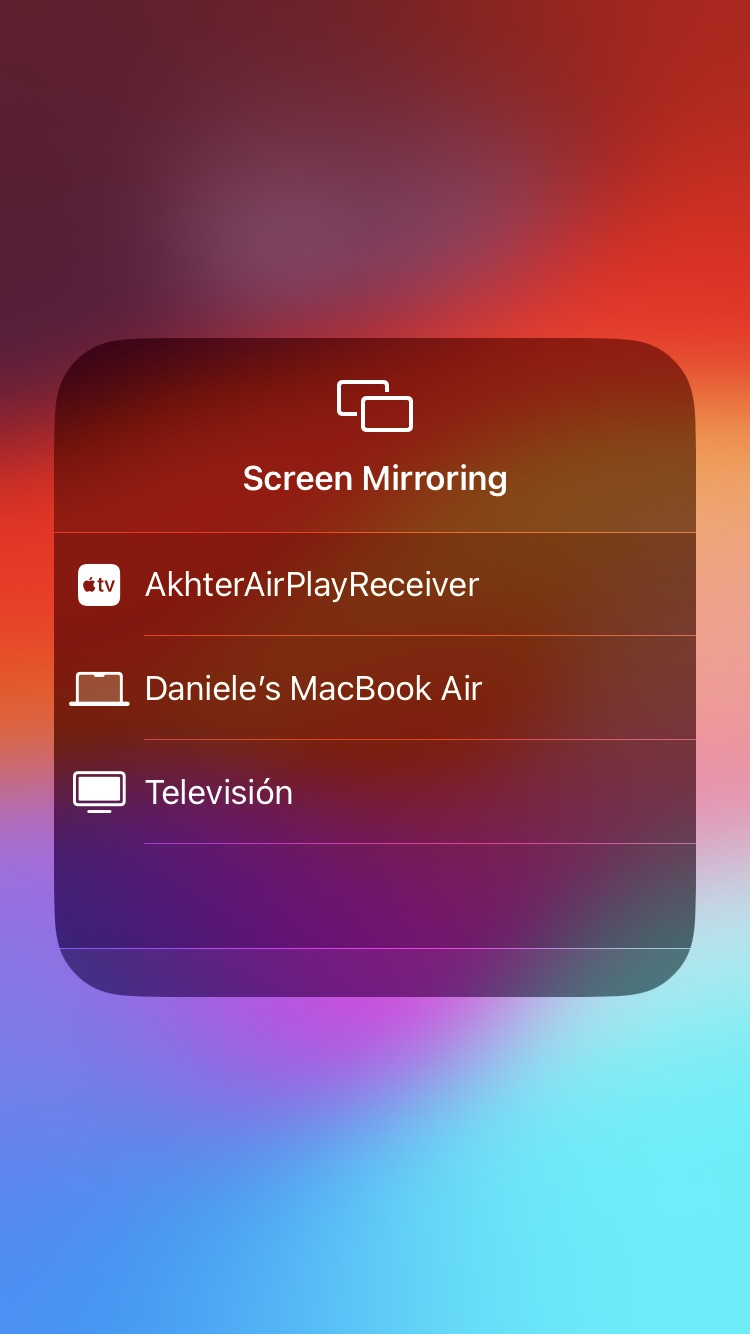
\includegraphics[width=4cm]{./chapters/iPhoneDetecting.jpeg}
    \caption{Representation of iPhone detecting Android device with Bonjour service.}\label{fig:iPhone-detecting}
  \end{wrapfigure}

  Our approach begins with the correct setup of Bonjour on the Android device, defining a JSON response containing essential parameters that describe the device and its capabilities. Initial investigation has highlighted several key parameters that must be included for successful device identification and connection initiation by an iOS device.
  The JSON response, typically returned when the iPhone queries the Bonjour service, needs to specify fields such as \texttt{deviceid}, \texttt{features}, \texttt{flags}, \texttt{model}, and \texttt{srcvers}. These parameters convey the device's unique identity, the capabilities it supports (e.g., AirPlay mirroring), and the protocol versions in use. By accurately configuring these fields, we aim to ensure the Android device can mimic the characteristics of a compatible AirPlay receiver, which are generally expected by iOS.
  Currently, our setup includes a simulated JSON configuration that imitates an AppleTV device, utilizing \texttt{model} values like \texttt{"AppleTV3,2"} and feature flags that signify support for AirPlay mirroring. This configuration has enabled preliminary recognition by the iPhone, but further tests are ongoing to validate full compatibility and to understand the response from the iOS device upon attempting to initiate a mirroring session.
%{\color{teal!90}\chapter{XMG6780A-V2 Firmware Update}\label{cap:XMG6780A-V2}}

\AddToShipoutPictureBG*{%
  \AtPageUpperLeft{%
    \raisebox{-\height}{%
      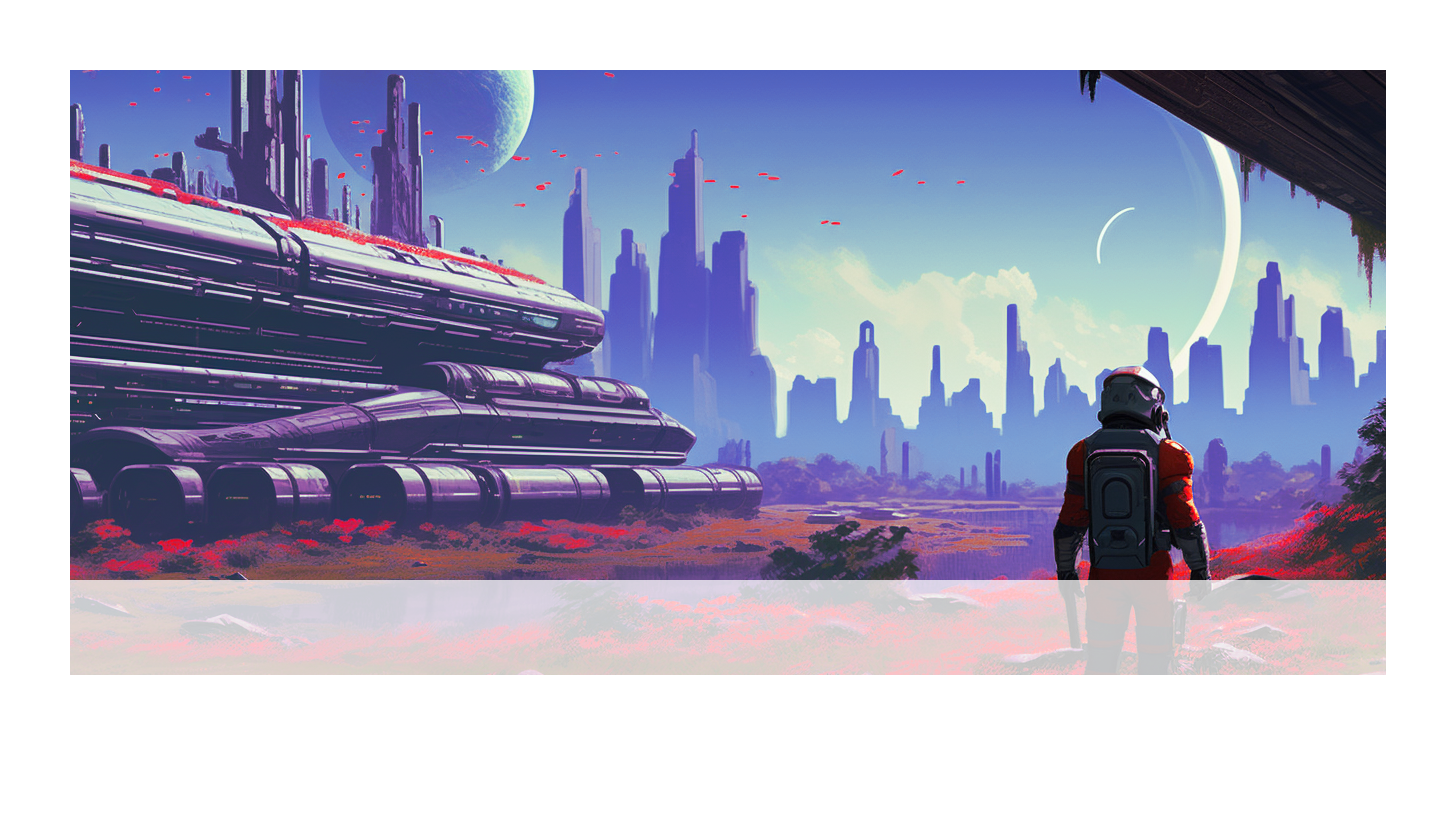
\includegraphics[width=\paperwidth]{./chapters/XMG6780A-V2.png}%
    }%
  }
}

\minitoc% Creating an actual minitoc mini lista contenuti


\section{XMG6780A-V2 Firmware}

After installing the \href{https://www.dropbox.com/scl/fi/razk4d533kkrign0e0kd1/wetransfer_new-firmware_2023-09-04_0553.zip?rlkey=jrls1bpkyo93ul3i0t1nokexu&dl=0}{XMG6780A-V2} firmware on the device, new customization options arise, including the ability to replace the default Launcher3 with a custom launcher. The limitations outlined in Cap. \ref{cap:resetting} encountered in the firmware originally present on the device at the time of Akhter's purchase on 08-08-2023, can be overcome by using the XMG6780A-V2 firmware.

\medskip
Once the custom launcher is configured as the default home, the issue of infinite boot-loop upon reboot is resolved. However, a problem might arise where the default launcher continues to appear despite the HOME action redirecting to the actual new custom launcher.

To resolve this issue, it's necessary to disable the default launcher3 using \cmd{\color{BrickRed}pm disable} for the \texttt{\color{BrickRed}com.xbh.launcher.overlay} and \texttt{\color{BrickRed}com.xbh.launcher} apps.

However, using the \texttt{\color{BrickRed}pm disable} in Android app would require root access. So we can either install the root firmware the Havistouch team provided us with, or we can use the \texttt{\color{BrickRed}hide} counterpart of \textbf{\color{BrickRed}devicepolicymanager} within our \emph{Taishan Tweaker} custom launcher.

With the intention of developing a new functional launcher, the idea is to create an in-app setup sequence. This sequence will guide us through the various steps that must be executed in the correct order:

\subsection{In-App Setup Sequence}

\begin{enumerate}
    \item set IP to \ipnum{\taishanIP}
    \item install \gls{shizuku} from the USB Kioxia drive
    \item install \gls{termux} from \href{https://github.com/danieledellacioppa/termux-app}{my fork}
    \item \cmd{adb connect \taishanIP}
    \item \faPlayCircle Install Taishan Tweaker
    \item Execute \cmd{adb shell dpm set-device-owner}\footnote{\label{dpm-enable-command} The full syntax is \texttt{\color{BrickRed}adb -s 192.168.11.207 shell dpm set-device-owner com.akhter.taishantweaker/.receivers.admin.AdminReceiver}}
        \begin{enumerate}
            \item{Now launch manually\footnote{\label{manually}Sometimes, the app remains on without the need for manual launch. This change occurred because, since 2023-10-05, the AdminReceiver triggers the SetupActivity to launch the MainActivity, whereas previously it used to directly launch the MainActivity leading the SetupActivity to crash systematically.} the Taishan Tweaker app}
            \item{Allow access to foto and media}
            \item{\faIcon{map-marker-alt} Location needs to be allowed at all times, otherwise it's a security risk. So for the time being, part of the setup involves going in Developer Settings and allowing this permission and set it to {\color{Bluetto}\faIcon{toggle-on} \android{Allow all the time}}}
            \item{The background will turn white.\footnote{\label{background-white} I've noticed that sometimes it doesn't and goes straight to the default one}}
        \end{enumerate}
    \item Set the custom launcher as default
        \begin{enumerate}
            \item The \faImage background will be the default one. Meaning the wall0.jpg which has index 0 in the list of wallpapers held by MyWallpaperManager
        \end{enumerate}
    \item Apply Tweaks
        \begin{enumerate}
            \item Always check that the Default Launcher option doesn't show Launcher3 anymore
            \item Also check Office WPS is actually gone
        \end{enumerate}
    \item Reboot
    \item Stop the Kiosk or enable everything via SAF
    \item Create a Google account
    \begin{enumerate}
        \item{This means going to Settings -> System -> About -> Click 10 times on About label -> Debug -> Enable Google Play Services}
        \item Open Google Play Store \faGooglePlay
        \item Might crash the first time
        \item Open again and log in with
        \begin{enumerate}
            \item{email: npcguillemruiz@gmail.com}
            \item{password: j4m3sbondwillr3turn}
        \end{enumerate}
        \item You should see the list of apps that are available for download
        \item {\color{BrickRed}\faWrench} Update all the apps via the Play Store
    \end{enumerate}
    \item Go back to the Taishan Tweaker and Install the keyboard\faKeyboard
    \begin{enumerate}
        \item{This will open the Play Store \faGooglePlay \ on the Gboard page}
        \item{\faPlayCircle Install}
        \item Don't open it yet
    \end{enumerate}
    \item Set Gboard as the default keyboard\faKeyboard
    \item Disable SmartIME
    \item Reboot
    \item Go back to the Taishan Tweaker and you should be all set to ship it to the customer
\end{enumerate}

\section{Replicating the CTOUCH Launcher Solution}

Since this touchscreen is different, rebuilding everything is necessary. The Android 8 CTOUCH Solution cannot be reused as it proves to be too unpredictable. The steps for this replication could be as follows:

\begin{enumerate}
    \item Setting up the Kiosk mode.
        \begin{enumerate}
            \item Maintaining an updated list of allowed packages.
                \begin{enumerate}
                    \item{Looking at violations attempt in Lock Task can give me the name of the package I want to enable}
                    \item{Translating the whole admin module is too much. I'm just doing an app\_lister button for now}
                \end{enumerate}
            \item onResume the kioskmode is set everytime. Is this what I want? \footnote{\label{onResume} for example when I launch the calculator the onResume is called and the kioskmode is set again.}
            \item Refer to the \textbf{central entity}\footnote{\label{central-entity} The central entity is a Class encapsulating a DevicePolicyManager, named MyDevicePolicyManager, which is injected via Dagger2.} that stores the complete list (as discussed in Section~\ref{sec:kiosk}) to prevent unexpected behavior.
            \item Ensure that the \textbf{central entity}\footref{central-entity} is the only one used throughout the program, as opposed to using a naked devicePolicyManager, which could lead to inconsistency. But because Dagger2 works only with activities we can't inject directly in AdminReceiver. It needs to pass through the MainActivity
        \end{enumerate}
    \item Configuring \gls{saf}\footnote{\label{SAF} Secure Access Framework} to enable challenge password functionality.
          \begin{enumerate}
              \item USBDetector now detects ProductID and VendorID
              \item UsbAttachReceiver that listens for Broadcasts when a USB is attached or detached. This class tries to put loginComplete to false when a USB is detached. This is not working yet. It'll be useful for \gls{saf}
              \item \gls{saf} is making use of shared preferences in a weird way...maybe I need a \textbf{central class} to handle all the shared preferences
          \end{enumerate}
    \item Creating a recyclerView to display applications.
    \item Disabling the sidebar\footnote{\label{sidebar} Ensuring that apps are only accessible via TaishanTweaker}
        \begin{enumerate}
            \item {\gls{navisettings} is the name of the floating sidebar that can be disabled. The question is: can I create a floating bar from my app to create/handle events like onBackPressed, Recents, PowerOFF, Reboot, etc..?}
            \begin{enumerate}
                \item{\gls{navisettings} might be actually part of the system and I could adjust the look accordingly. This way I can post-pone recyclerView implementation. Also I won't have to create a floating bar to navigate.}
            \end{enumerate}
        \end{enumerate}
    \item Adding buttons in the \gls{ui} to control Wi-Fi\faWifi, Bluetooth\faBluetooth \footnote{\label{blue-not-needed} Invoking the getInstalledApplications(PackageManager.GET\_META\_DATA) method on an instance of the PackageManager class, returns a list of all the installed applications. This list includes the Bluetooth app. This means that Bluetooth can be disabled already without having to write any code.}, screenshots, and USB\faHdd \ functionality.
    \begin{enumerate}
        \item We should consider registering a BroadcastReceiver to \emph{android.net.conn.CONNECTIVITY\_CHANGE} to detect when the device is connected to the internet. At the moment, this is being done by launching a service that shuts the wifi periodically. This is not ideal.
        \begin{enumerate}
            \item{We found a package called \textbf{com.android.networkstack} that is both responsible for the Wi-Fi and the Ethernet. We can disable it. There will be a reboot. And both Wi-Fi and Ethernet will be disabled.}
        \end{enumerate}
        \item Bluetooth is not needed. It can be disabled already by disabling \emph{com.android.bluetooth} in the \textbf{Package Disabler}.
        \item Screenshots is part of the USB button. I need to split it.
        \item USB has a proper button now to enable/disable it. I need to add the functionality to take screenshots.
    \end{enumerate}
    \item Make the app lighter by removing unnecessary code. There are several performance issues that need to be addressed.
\end{enumerate}

\clearpage
\subsection{Kiosk}
\label{sec:kiosk}

To ensure proper functionality, it's essential to have a \textbf{central entity}\footref{central-entity} that globally stores the complete updated list of allowed packages. Otherwise, running the command at line \ref{lockArray} of the Listing \ref{lst:kioskfun} in the future may result in packet loss and lead to unexpected behaviors that are challenging to debug.

\lstinputlisting[language=Kotlin,linewidth=0.8\linewidth,caption={Kiosk Function}, label=lst:kioskfun, escapechar=\%]{./chapters/code/kioskfun.kt}

\subsection{Hiding packages}

Using the devicePolicyManager to hide packages can create problems. Here comes the list of packages that you shouldn't hide:

\begin{itemize}
    \item android
    \begin{enumerate}
        \item This package if allowed you'll be able to shutdown during Kiosk mode. If you disable it, you won't be able to shutdown at all. I'll keep it away from the list of packages to hide.
    \end{enumerate}
    \item android.ext.services
        \begin{enumerate}
            \item The system remains stable if you disable it. The issue is, this is a module that updates framework components for core Android OS functionality. These components include services for managing notifications, text auto-complete matching strategies, storage cache, and other services that run continuously. The module is updatable, meaning it can receive updates to functionality outside of the normal Android release cycle. Is autocompletion a requirement for the user? If so, then we can't disable it. For now I'll keep it away from the list of packages to hide.
        \end{enumerate}
    \item android.ext.shared
        \begin{enumerate}
            \item The system remains stable if you disable it. I don't what it does but it's probably related to the previous package. I'll keep it away from the list of packages to hide.
        \end{enumerate}
    \item com.android.apps.tag
        \begin{enumerate}
            \item The system remains stable if you disable it. It's the NFC app? I'll keep it away from the list of packages to hide.
        \end{enumerate}
    \item com.android.backupconfirm
        \begin{enumerate}
            \item The system remains stable if you disable it. It's belonging to the dialog popping up when initiating adb backup, and which does nothing but asking you to confirm whether the remotely triggered backup should be executed (and if you want to protect it with a password). I'll keep it away from the list of packages to hide.
        \end{enumerate}
    \item com.android.bips
        \begin{enumerate}
            \item The system remains stable if you disable it. It's the Bluetooth Input Profile Service. I'll keep it away from the list of packages to hide.
        \end{enumerate}
    \item com.android.bluetoothmidiservice
        \begin{enumerate}
            \item The system remains stable if you disable it. It's the Bluetooth MIDI Service. I'll keep it away from the list of packages to hide.
        \end{enumerate}
    \item com.android.bluetooth
        \begin{enumerate}
            \item This packet seems like it's doing the same thing I've done on CTOUCH Android 8. It's a service that runs in the background and it's responsible for the Bluetooth functionality. If you disable it, you won't be able to turn on Bluetooth again. I'll definitely keep it as an option for the user to enable/disable.
        \end{enumerate}
    \item com.android.cameraextensions
        \begin{enumerate}
            \item The system remains stable if you disable it. In low light scenarios, the camera app will automatically switch to night mode. I'll keep it away from the list of packages to hide.
        \end{enumerate}
    \item com.android.systemui
        \begin{enumerate}
            \item The system goes black.
            \item You can't unhide it since it'll give you the outpout shown at line n. \ref{systemui_out} of the Listing \ref{lst:unhidesystemui}.
            \item It remains hidden anyway. One way to recover is via \cmd{\color{BrickRed} adb shell reboot recovery}
        \end{enumerate}
\end{itemize}

\lstinputlisting[language=bash,linewidth=0.8\linewidth,caption={Unhiding SystemUI}, label=lst:unhidesystemui, escapechar=\%]{./chapters/code/unhide_android_systemui}

\begin{itemize}

    \item com.android.settings
    \item com.android.providers.set
    \item com.android.providers.settings
    \item com.android.providers.userdictionary
    \item com.android.providers.contacts
    \item com.android.providers.media
    \item com.android.providers.downloads
    \item com.xbh.share
        \begin{enumerate}
            \item This is AirgoCast and takes advantage when the app crashes so for security reasons it's disabled for now
        \end{enumerate}
\end{itemize}








%{\color{teal!90}\chapter{XMA311D2A-2-V1 Firmware Structure}\label{cap:xma311d2a-2-v1}}

\AddToShipoutPictureBG*{%
  \AtPageUpperLeft{%
    \raisebox{-\height}{%
      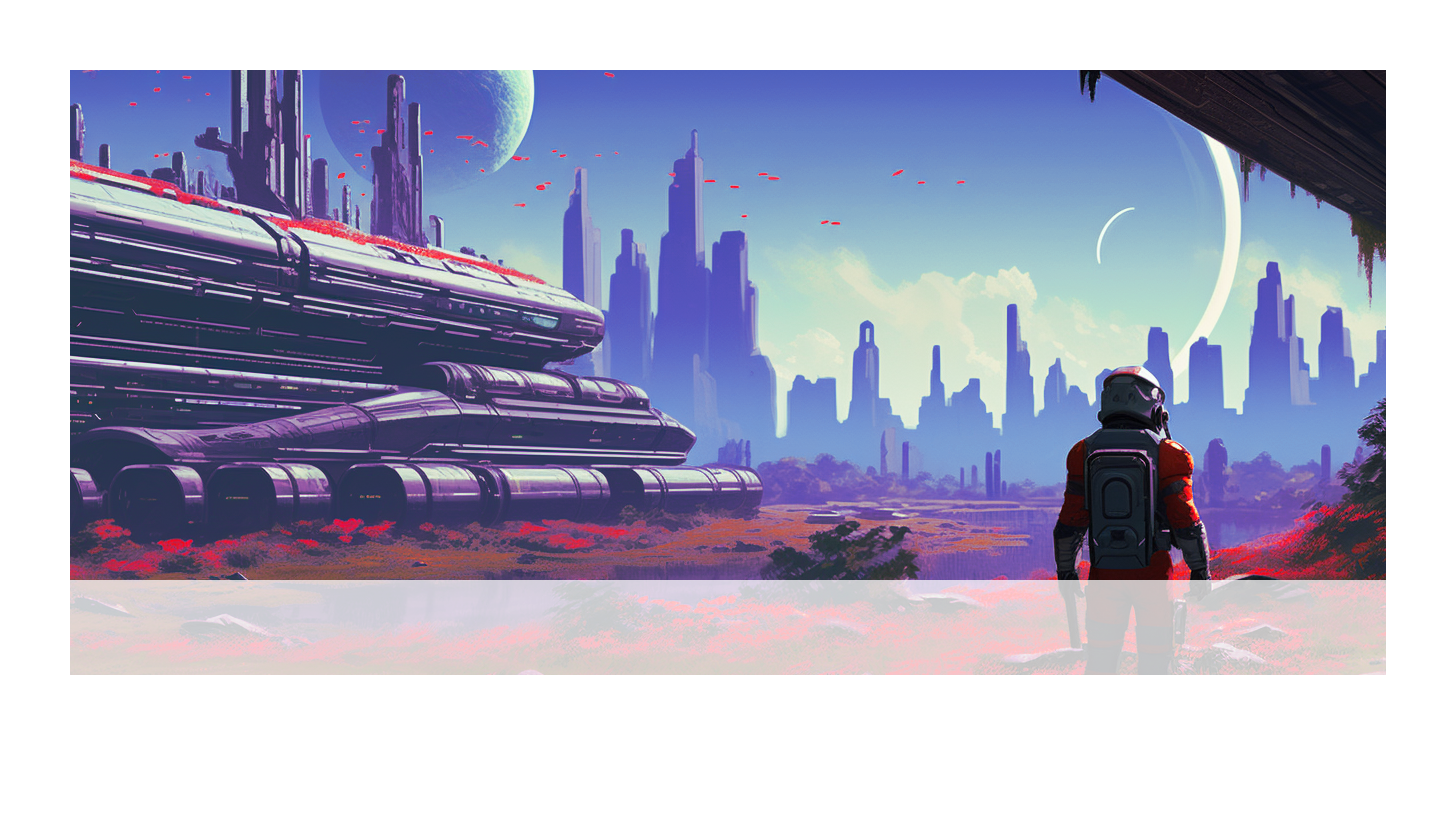
\includegraphics[width=\paperwidth]{./chapters/XMG6780A-V2.png}%
    }%
  }
}

\minitoc% Creating an actual minitoc mini lista contenuti


\section{XMA311D2A-2-V1 Firmware}
At page n. \pageref{tab:xma311d2a-2-v1-binwalk} we show the \gls{binarywalk} of the XMA311D2A-2-V1 firmware. The firmware is a 3.6 GB file.
It's probably an archive file, but we can't be sure. Many info will be useful in case we want to
flash our own OS.

% small text from now on
\scriptsize
\begin{landscape}
\input{./chapters/imagewalktable.tex}
\end{landscape}
\normalsize

\section{Some system properties}
%\input{./getproperties/getProperties/getprop.tex}

\clearpage
\section{Creating a custom firmware}
In Table \ref{tab:cpuinfo} it is shown the output of the command {\color{BrickRed}\texttt{adb shell cat /proc/cpuinfo}} which obtains the details of the CPU cores.
To gather additional system information I'm using the command {\color{BrickRed}\texttt{adb shell getprop}} (see Listing \ref{lst:adbshellgetprop}), thus obtaining further mission critical system details:

\lstinputlisting[language=bash,linewidth=0.8\linewidth,caption={adb shell getprop}, label=lst:adbshellgetprop, escapechar=\%]{./chapters/code/critical_sys_info.txt}

\subsubsection{Significance of \texttt{ro.board.platform} = \texttt{t7} for Custom Firmware Development}

The value \texttt{ro.board.platform} indicating \texttt{t7} provides critical information regarding the specific \gls{SoC} or hardware platform that the device is based on. Understanding this value is essential as it directly impacts the development and customization of the firmware.

\paragraph{Identification of the SoC}
The \texttt{t7} value typically corresponds to a particular \gls{SoC} model used in the device. This identifier is crucial because it defines the hardware characteristics, such as the type of CPU, GPU, memory controllers, and other integrated components. Knowing that the device is built on the \texttt{t7} platform allows us to search for specific documentation, drivers, and resources in the Linux kernel or Android Open Source Project (AOSP) that are compatible with this platform.

\paragraph{Kernel and Driver Compatibility}
The \texttt{t7} platform requires a kernel that fully supports all features of the \gls{SoC}. This means the kernel must include the necessary drivers for the processor, GPU, memory controller, and other critical components. During the development of the custom firmware, it will be necessary to ensure that the selected or modified kernel is optimized for the \texttt{t7} platform. Failure to do so may result in hardware features not functioning correctly or at all.

\paragraph{ARM Architecture Support}
Given that the \texttt{t7} platform is associated with a 64-bit ARM architecture (\texttt{arm64-v8a}), it is imperative to ensure that the firmware is built with support for ARMv8-A. This includes extensions such as NEON for SIMD (Single Instruction, Multiple Data) processing and other architecture-specific optimizations. The firmware will also need to manage compatibility with 32-bit applications (\texttt{armeabi-v7a} and \texttt{armeabi}), which may still be in use, especially in legacy environments.

\paragraph{Customization and Optimization}
Knowing that the platform is \texttt{t7} allows us to make platform-specific optimizations, such as power management, memory allocation, and thermal performance, which are crucial for embedded devices or low-power systems. Customizing the firmware for \texttt{t7} may involve integrating specific software or middleware that takes advantage of the unique hardware capabilities of the platform, thereby enhancing overall efficiency and performance.

\paragraph{Research and Community Support}
Since the device utilizes the \texttt{t7} platform, we can explore online communities, open-source code repositories, and documentation specific to this platform, making problem-solving and resource gathering more efficient. If \texttt{t7} is a common platform, there may already be existing work on custom firmware or optimized kernels that can serve as a foundation for our project.

\subparagraph{Next Steps}
\begin{enumerate}
  \item **Documentation and Research**: Begin by thoroughly researching \texttt{t7}, seeking technical specifications, \gls{SoC} documentation, and any available resources through forums or open-source project repositories.
  \item **Kernel Selection**: Base the custom firmware's kernel on a version that fully supports the \texttt{t7} platform, applying any necessary patches or modifications to ensure optimal device support.
  \item **Development and Testing**: During firmware development, rigorous testing is crucial to ensure that all hardware components supported by the \texttt{t7} platform function as expected, including support for both 32-bit and 64-bit applications.
\end{enumerate}

This approach will ensure that the custom firmware is perfectly adapted to the specific hardware platform of the device, maximizing system performance and stability.


%\clearpage
\begin{table}
  \centering
  \scriptsize
  \begin{tabular}{|c|c|c|c|c|c|c|c|}
    \hline
    \textbf{Processor} & \textbf{BogoMIPS} & \textbf{Features} & \textbf{CPU Implementer} & \textbf{CPU Architecture} & \textbf{CPU Variant} & \textbf{CPU Part} & \textbf{CPU Revision} \\ \hline
    0 & 48.00 & fp, asimd, evtstrm, aes, pmull, sha1, sha2, crc32, cpuid & 0x41 & 8 & 0x0 & 0xd09 & 2 \\ \hline
    1 & 48.00 & fp, asimd, evtstrm, aes, pmull, sha1, sha2, crc32, cpuid & 0x41 & 8 & 0x0 & 0xd09 & 2 \\ \hline
    2 & 48.00 & fp, asimd, evtstrm, aes, pmull, sha1, sha2, crc32, cpuid & 0x41 & 8 & 0x0 & 0xd09 & 2 \\ \hline
    3 & 48.00 & fp, asimd, evtstrm, aes, pmull, sha1, sha2, crc32, cpuid & 0x41 & 8 & 0x0 & 0xd09 & 2 \\ \hline
    4 & 48.00 & fp, asimd, evtstrm, aes, pmull, sha1, sha2, crc32, cpuid & 0x41 & 8 & 0x0 & 0xd03 & 4 \\ \hline
    5 & 48.00 & fp, asimd, evtstrm, aes, pmull, sha1, sha2, crc32, cpuid & 0x41 & 8 & 0x0 & 0xd03 & 4 \\ \hline
    6 & 48.00 & fp, asimd, evtstrm, aes, pmull, sha1, sha2, crc32, cpuid & 0x41 & 8 & 0x0 & 0xd03 & 4 \\ \hline
    7 & 48.00 & fp, asimd, evtstrm, aes, pmull, sha1, sha2, crc32, cpuid & 0x41 & 8 & 0x0 & 0xd03 & 4 \\ \hline
  \end{tabular}
  \caption{Details of the CPU cores obtained from \texttt{adb shell cat /proc/cpuinfo}.}
  \label{tab:cpuinfo}
\end{table}

\begin{itemize}
  \item \textbf{fp}: Floating Point Unit, responsible for handling arithmetic operations on floating-point numbers, crucial for scientific calculations and multimedia processing.
  \item \textbf{asimd}: Advanced SIMD (Single Instruction, Multiple Data), also known as NEON, enables parallel processing, essential for tasks like signal processing and multimedia encoding.
  \item \textbf{evtstrm}: Event Stream, allows the processor to efficiently handle sequences of operations or events, used in real-time processing applications.
  \item \textbf{aes}: Advanced Encryption Standard, a widely used symmetric encryption algorithm for securing data, recognized for its efficiency in both hardware and software.
  \item \textbf{pmull}: Polynomial Multiply, an instruction that accelerates polynomial arithmetic, useful in cryptographic applications like Galois/Counter Mode (GCM).
  \item \textbf{sha1}: Secure Hash Algorithm 1, produces a 160-bit hash value, used for data integrity verification and digital signatures.
  \item \textbf{sha2}: Secure Hash Algorithm 2, a family of cryptographic hash functions producing 224, 256, 384, or 512-bit hash values, used in security protocols like SSL/TLS.
  \item \textbf{crc32}: Cyclic Redundancy Check 32-bit, an error-detecting code used to check data integrity, widely implemented in network communications and file storage systems.
  \item \textbf{cpuid}: CPU IDentification, an instruction that provides details about the processor's type, capabilities, and features, essential for optimizing software.
  \item \textbf{0x41}: Hexadecimal value identifying the CPU implementer, which corresponds to ARM Ltd., the designer of the ARM architecture.
  \item \textbf{CPU Architecture}: Refers to the processor's underlying design, where '8' indicates ARMv8-A, a 64-bit architecture used in modern devices.
  \item \textbf{CPU Variant}: A specific version or model of the CPU core within a broader architecture family, indicating different iterations with possible feature variations.
  \item \textbf{CPU Part}: A unique identifier for a specific CPU core, such as 0xd09 for Cortex-A53 and 0xd03 for Cortex-A55, distinguishing cores with different performance characteristics.
  \item \textbf{CPU Revision}: The revision number of the CPU core, indicating specific version updates that may include bug fixes or performance enhancements.
\end{itemize}

\section{Outcome and Next Steps}
As of 14 Aug 2024, we have successfully determined the CPU architecture and key features of the XMA311D2A-2-V1 device. These details confirm that the device is built on the ARMv8-A architecture, specifically utilizing Cortex-A53 and Cortex-A55 cores.

\subsection{Next Steps}
Based on this information, our immediate next steps will include:

\begin{enumerate}
  \item \textbf{Identifying a Compatible AOSP Version}: We'll begin by locating a version of the Android Open Source Project (AOSP) that is compatible with ARMv8-A architecture and supports the specific features of the Cortex-A53 and Cortex-A55 cores.
  \item \textbf{Custom Kernel Development}: Given the specifics of the hardware, we will explore the kernel sources provided by ARM and potentially modify them to suit the custom needs of our firmware, ensuring support for all critical features like AES encryption and advanced SIMD operations.
  \item \textbf{Cross-Compiling the Firmware}: Once we have a compatible version of AOSP, we will proceed with cross-compiling the custom firmware. This will involve integrating necessary drivers and ensuring compatibility with the device's hardware.
  \item \textbf{Testing and Validation}: After compiling the custom firmware, we will perform rigorous testing on a single device to validate the stability and functionality of the firmware before rolling it out across all 70 screens.
  \item \textbf{Documentation and Process Refinement}: We will document the entire process and refine our approach based on the outcomes of the testing phase, ensuring that we have a robust method for future firmware updates or custom builds.
\end{enumerate}

By following these steps, we aim to develop a stable and reliable custom firmware that fully leverages the hardware capabilities of the XMA311D2A-2-V1, while also laying the groundwork for future enhancements and updates.
%{\color{teal!90}\chapter{User Interface}\label{cap:ui}}

\AddToShipoutPictureBG*{%
  \AtPageUpperLeft{%
    \raisebox{-\height}{%
      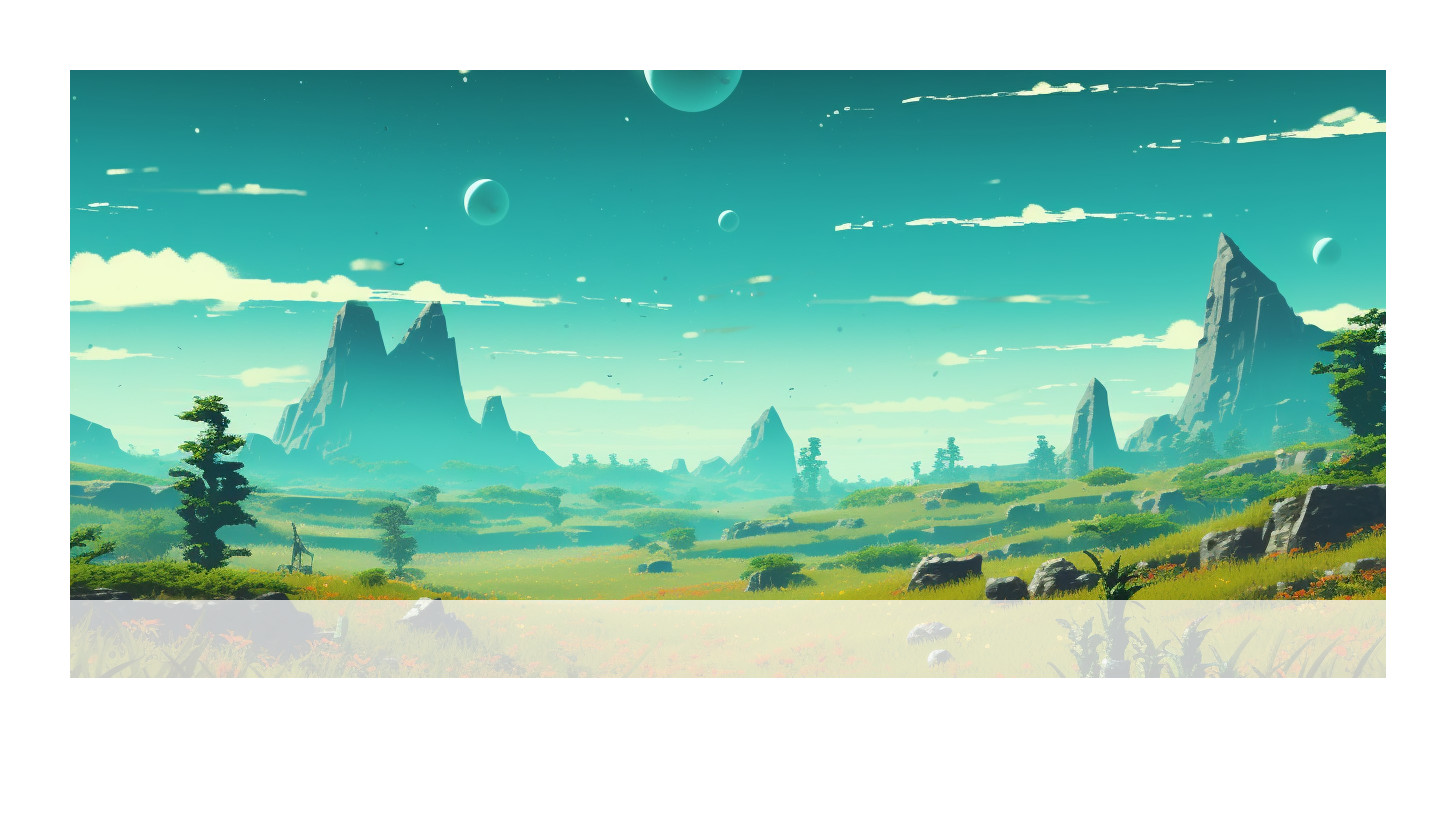
\includegraphics[width=\paperwidth]{./chapters/user-interface.jpg}%
    }%
  }
}

\minitoc% Creating an actual minitoc mini lista contenuti


\section{The Look}

\simplewrap{13}{R}{8cm}{8cm}{./chapters/user-interface/ui-clock.png}{-10pt}{Temporary Prototype of the \gls{ui} showing clock and console}{fig:clock}

On September 7\textsuperscript{th}, after re-enabling \gls{navisettings}, which serves as the system app for navigation and other functions, I made some notable visual adjustments (fig. \ref{fig:clock}):

\begin{enumerate}
    \item I relocated the console (which will eventually transform into a widget) to the side of the app's interface. This change allows for a cleaner main view and opens up more space for other essential features.
    
    \item I introduced a dedicated view to display the current time, with updates occurring every 1000 milliseconds (1 second). This time-display functionality is managed by a class named \texttt{TimeUpdater}. Notably, this class was integrated using Dagger2 for dependency injection, eliminating the need for direct \texttt{findViewById(R.id.timeTextView)} usage in \texttt{MainActivity.kt}.
\end{enumerate}

These alterations contribute to an improved app appearance and functionality. The console's new side placement offers convenience, and the real-time clock display, powered by \texttt{TimeUpdater} and managed through Dagger2, enhances the user experience.

\clearpage
\subsection{2023-09-08 update}
\simplewrap{13}{R}{8cm}{8cm}{./chapters/user-interface/ui-central-clock.jpg}{-10pt}{Improved resolution of the \gls{ui} showing clock at the center}{fig:central-clock}

I have made some more changes to the UI, as shown in figure \ref{fig:central-clock}. The clock is now at the center of the screen, and the console is on the right side. I have also added a background image, which is the same as the system wallpaper. This is a temporary solution to the wallpaper issue, which I will address later in this chapter.

\medskip
Also the clock is now updating every minute, instead of every second. This still didn't resolve the lag issue. I will need to investigate further.

\clearpage
\section{settingsButtonClickListener}
The injection shown in Listing \ref{lst:weird-injection} keeps the MainActivity cleaner, but it may seem unconventional as the injected object is never directly used. It returns a listener, which, in this case, isn't utilized since all the initialization is done during build time. Is this the right approach? While it serves its purpose, one might question if it aligns with best practices.
\lstinputlisting[language=Kotlin,linewidth=0.8\linewidth,caption={Weird Injection}, label=lst:weird-injection, escapechar=\%]{./chapters/code/weird-injection.kt}

\section{Wallpaper}
Even though this app is now the default launcher, the wallpaper displayed on boot differs from what's expected. To temporarily address this issue, I have applied a single image as both the system wallpaper and the app layout background. However, there is significant work ahead in translating the Java code from the CTOUCH project to Kotlin for the Taishan project. This includes implementing policies using SharedPreferences to allow users to change the wallpaper and make it permanent once selected. Currently, this is just for a quick look, as other more pressing matters demand my attention. Therefore, I'll tackle this aspect towards the end of the project.

\subsection{Wallpaper Resolution}
I did upscale the image to 5824x3264, which is higher than Taishan's resolution. This is to ensure that the image is not stretched or distorted when displayed on the screen. However, this is not the optimal solution, as it increases the app's size. I will need to find a way to downscale the image to the correct resolution without compromising the image quality.
Maybe even performances could be affected by this, but I will need to test this hypothesis. Or maybe it's the clock updating every second that is causing the lag.

\section{The DebugConsole}
The DebugConsole is now a widget that can be moved around the screen. It can't be resized yet, but it can be moved around. It disappears and appears on demand by clicking the \texttt{Shell Button}\footnote{The Shell Button is handled with \textbf{ConsoleToggleButtonClickListener} which is injected in the MainActivity.kt using Dagger2.}.

\section{The Recycler View}
The Recycler View is now working. It displays a list of all the features that are currently implemented. Injections are also working, and the code is cleaner.

\section{Features Implemented}
\begin{itemize}
    \item \textbf{Clock} - The clock is now at the center of the screen. It updates every minute. It is powered by \textbf{TimeUpdater} and managed through \gls{dagger2}.
    \item \textbf{DebugConsole} - The DebugConsole is now a widget that can be moved around the screen. It can't be resized yet, but it can be moved around. It disappears and appears on demand by clicking the \texttt{Shell Button}. It is managed through \gls{dagger2}.
    \item \textbf{App Drawer} - The App Drawer is now a Recycler View that displays a list of all the apps that are currently installed on the device. It is powered by \textbf{AppListAdapter} and managed through \gls{dagger2}.
    \begin{enumerate}
        \item \textbf{Launch it via Remote Control} - The App Drawer can be launched via the Remote Control by pressing the \faWindows\ button.
    \end{enumerate}
\end{itemize}
%{\color{teal!90}\chapter{Advanced configuration}\label{cap:advanced-configuration}}

\AddToShipoutPictureBG*{%
  \AtPageUpperLeft{%
    \raisebox{-\height}{%
      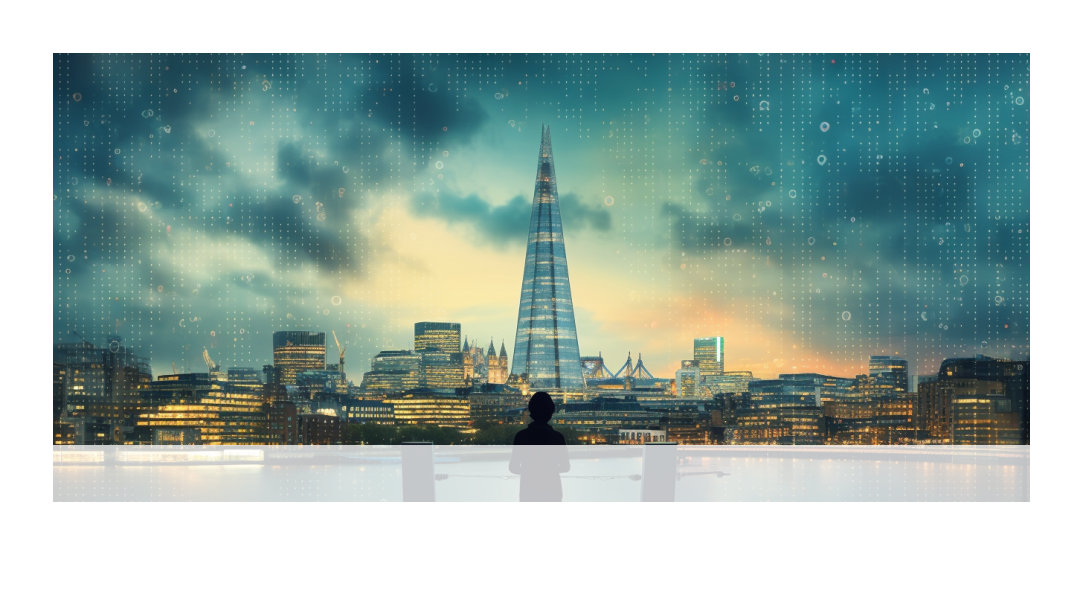
\includegraphics[width=\paperwidth]{./chapters/advanced-configuration.png}%
    }%
  }
}

\minitoc% Creating an actual minitoc mini lista contenuti


\section{Introduction}

In a context where we have configured an Android device in kiosk mode using the \gls{dpm} as a device owner, and we have implemented a custom launcher without access to settings for the end user, the action of setting up Termux and using its API to start Shizuku can be described as \emph{device preparation} or \emph{advanced configuration}

\medskip
\begin{center}
These actions \textbf{cannot} be considered {\color{BrickRed} \emph{a true privilege escalation}} in the traditional sense of the term
\end{center}
\medskip


This, is purely because we are configuring and using existing applications (Termux and Shizuku) to perform certain operations rather than gaining unauthorized or unintentional access at the system level. However, we are leveraging the features of Termux and Shizuku to perform advanced actions that would normally require root privileges or ADB commands. It's important to note that these actions should be clearly documented, and the device should be configured in compliance with company policies or device usage policies, especially considering its use in kiosk mode. Additionally, we should ensure that access to Termux and Shizuku is limited only to the necessary operations and that no security vulnerabilities are introduced that could compromise the stability or security of the kiosk device. In summary, while it's not a privilege escalation in the traditional sense, it is still an advanced device configuration that should be implemented carefully and appropriately documented.

For now we'll focus on the following actions:

\begin{itemize}
    \item Disabling keyboard and navigation overlays to make sure the device starts in a very protected state. The final user should never be able to use the terminal or navigate the device during boot sequence.
    \item Understanding what can we do with Shizuku now that is enabled. Why are they all claiming that Shizuku can call hidden APIs? How can we use them without having to use reflection?
    \item Use a service aware of the internal logcat to detect when termux is being launched so that we can start sending commands to it.
    \item Are there any termux commands that can be used to shut services down? For example, can we use termux to shut down the system UI?
    \item Can we make the gap shorter when we enable \gls{navisettings} temporarily? Can we make it so that it's only enabled for a few seconds?
    \begin{itemize}
        \item Can we actually have \gls{navisettings} enabled at all times and use Termux to make it secure?
    \end{itemize}
\end{itemize}
%{\color{teal!90}\chapter{How Does The Akhter Launcher work?}\label{cap:how-does-the-akhter-launcher-work}}

\AddToShipoutPictureBG*{%
  \AtPageUpperLeft{%
    \raisebox{-\height}{%
      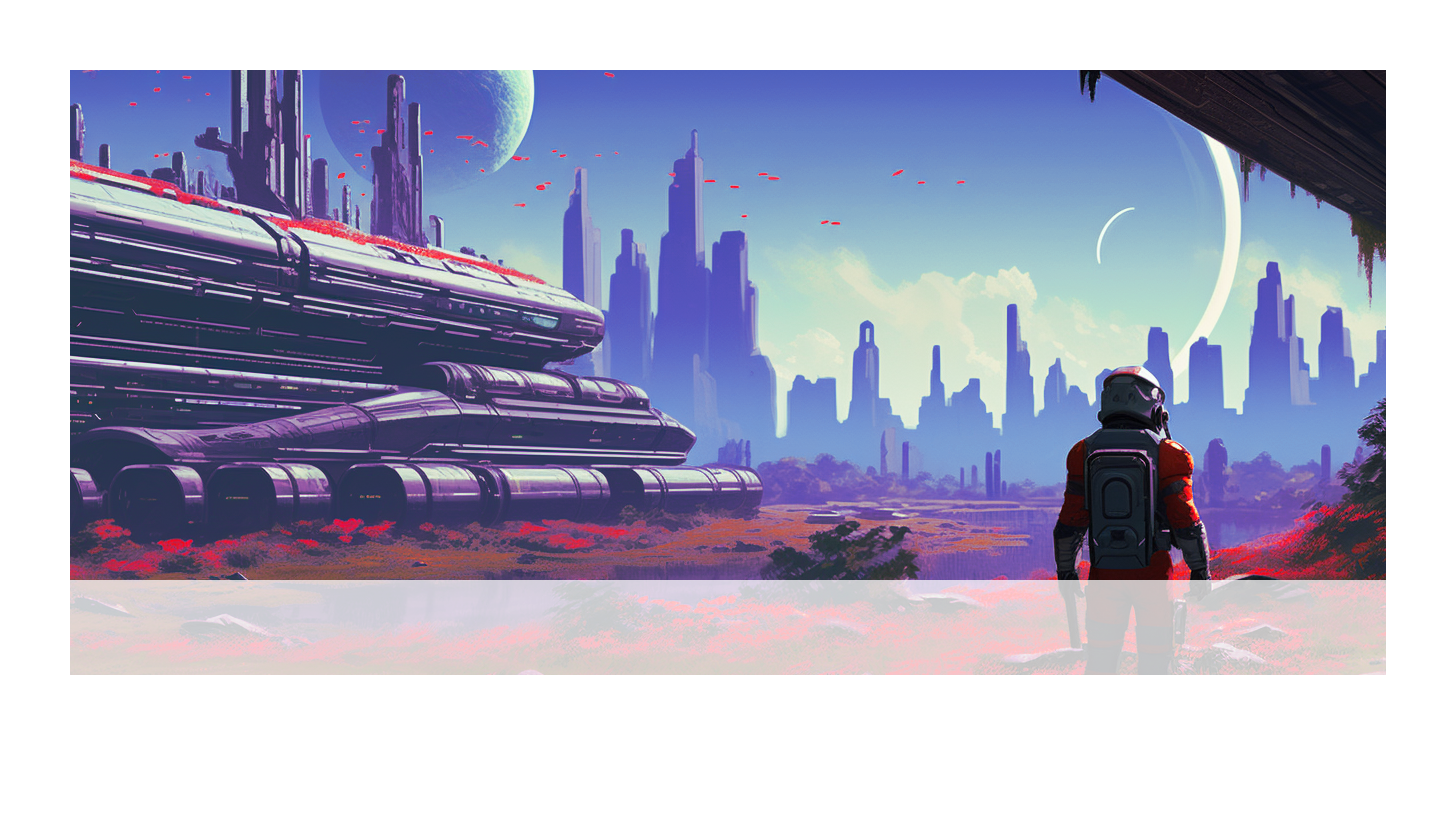
\includegraphics[width=\paperwidth]{./chapters/XMG6780A-V2.png}%
    }%
  }
}

\minitoc% Creating an actual minitoc mini lista contenuti

\section{USB Detection}\label{sec:usb-detection}
%  {\color{teal!90}\chapter{Changing Boot Animation}\label{cap:changing-boot-animation}}

  \AddToShipoutPictureBG*{%
    \AtPageUpperLeft{%
      \raisebox{-\height}{%
        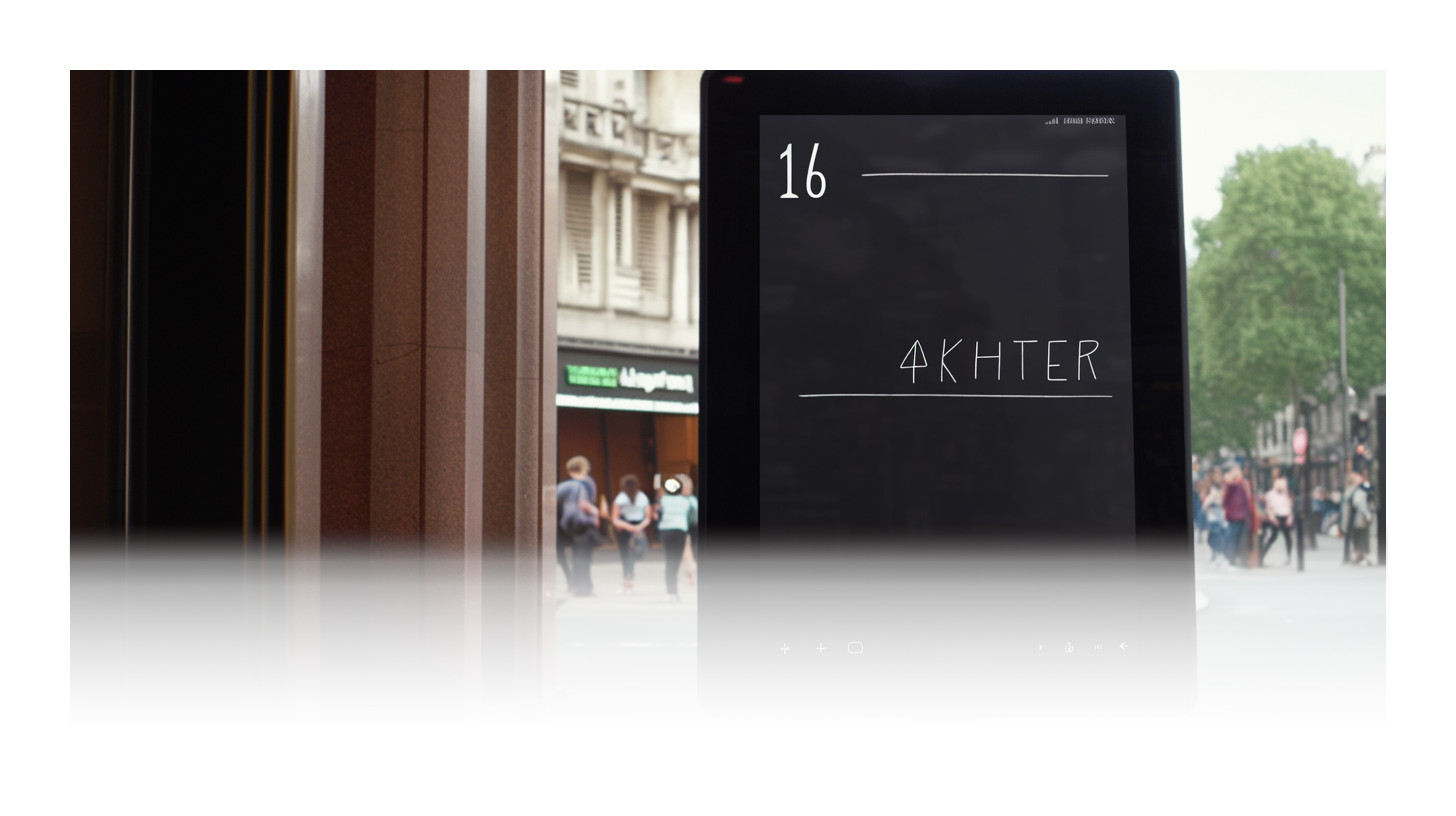
\includegraphics[width=\paperwidth]{./chapters/ifp_piccadilly.jpeg}%
      }%
    }
  }

  \minitoc% Creating an actual minitoc mini lista contenuti

  \section{Introduction}

  In this chapter, we will cover the steps required to customize the boot animation on a \gls{userdebug} device. This process involves creating a new boot animation, packaging it correctly, and using ADB commands to deploy it onto the device.

  \section{Creating the Boot Animation}

  The boot animation consists of multiple frames and a description file. For our device at Akhter Computers, the flat panel supports a maximum resolution of 2028x1126. The animation is generated in Blender and is divided into three parts:

  \begin{itemize}
    \item 81 frames in
    \begin{tikzpicture}[baseline=(text.base)]
      \node (icon) at (0, 0.3) {\color{Gray}\faIcon{folder-open}};
      \node (text) at (0, 0) {\desktopfile{akhter}};
    \end{tikzpicture}
    namely from 0 to 80. The first is called \desktopfile{fair\_00000.jpg} and the last \desktopfile{fair\_00080.jpg}

    \item 80 frames in
    \begin{tikzpicture}[baseline=(text.base)]
      \node (icon) at (0, 0.3) {\color{Gray}\faIcon{folder-open}};
      \node (text) at (0, 0) {\desktopfile{part1}};
    \end{tikzpicture}
    from 81 to 160. The first is called \desktopfile{00081.jpg} and the last \desktopfile{00160.jpg}

    \item A description in
    \begin{tikzpicture}[baseline=(text.base)]
      \node (icon) at (0, 0.3) {\color{Gray}\faIcon{file-alt}};
      \node (text) at (0, 0) {\desktopfile{desc.txt}};
    \end{tikzpicture}
    (cf. \ref{subsec:desc-txt})
  \end{itemize}

  The naming convention of the files seems to be very much free to choose in my opinion. The only requirement is that the files should be named in numerical order. The \desktopfile{desc.txt} file is used to manage the playback of the frames.

  \subsection{Description File - desc.txt}
  \label{subsec:desc-txt}

  The \emph{desc.txt} is managing the playback of the frames. This file is structured as follows:

  \begin{verbatim}
    2028 1126 30
    p 1 2 akhter
    p 0 0 part1
  \end{verbatim}

    \begin{itemize}
        \item `2028 1126 30`: Specifies the width, height, and \gls{fps} of the animation.
        \item `p 1 2 akhter`: Plays the frames in the "akhter" folder 1 time, with a 2-frame pause between loops.
        \item `p 0 0 part1`: Plays the frames in the "part1" folder indefinitely with no pause.
    \end{itemize}

  \subsection{Compressing the Boot Animation}

  To ensure the animation is displayed correctly, the compression factor must be set to 1.00. Use the following command to create the `bootanimation.zip`:


  \cmd{zip -r0 ./bootanimation.zip .}

  \section{Deploying the Boot Animation}

  Deploying the boot animation requires several ADB commands. This has been tested only on a \gls{userdebug} distro of Android.

  \subsection{Instructions \faCode}

  \begin{enumerate}
    \item Enable root access:

    \cmd{\faIcon{caret-right} adb root}

    \item Remount the system partition to make it writable:

    \cmd{\faIcon{caret-right} adb remount}

    \item Backup the existing boot animation:

    \cmd{\faIcon{caret-right} adb shell mv /product/media/bootanimation.zip /product/media/bootanimation.old.zip}

    \item Push the new boot animation to the device:

    \cmd{\faIcon{caret-right} adb push ./bootanimation.zip /product/media/bootanimation.zip}

    \item Sync the file system to ensure all changes are written:

    \cmd{\faIcon{caret-right} adb shell sync}
  \end{enumerate}
  \section{Conclusion}

  Customizing the boot animation on a userdebug device involves creating the animation frames, packaging them correctly, and using ADB commands to deploy the new animation. By following these steps, you can personalize the boot experience of your device.


%  \roundedwrap{19}{R}{0cm}{10cm}{./chapters/kioskTest_idea.png}{-10pt}{Kiosk Test Idea}{fig:kiosk-test-idea}{Black}

%  {\color{teal!90}\chapter{JUnit4 Test Plan}\label{cap:junit4-test-plan}}

  \AddToShipoutPictureBG*{%
    \AtPageUpperLeft{%
      \raisebox{-\height}{%
        
\includegraphics[width=\paperwidth]{./chapters/jUnit4_testing.jpeg}%
      }%
    }
  }

  \minitoc% Creating an actual minitoc mini lista contenuti

  \section{JUnit4 Test Plan}

  The most important test we need to plan is the Kiosk Test. In figure \ref{fig:kiosk-test-idea}, we show the idea of the test. The test will be performed on a Kiosk, and we will test the following:

  \section{Kiosk Mode Test Description}

  This test in JUnit4 needs to check the behavior of the \gls{ifp} Android device in Kiosk Mode (LockTask). The test objectives are as follows:

  \begin{enumerate}
    \item Verify that when the device is in LockTask mode, only the apps allowed to run in Kiosk Mode can be launched.
    \item Ensure that attempts to launch apps not allowed in LockTask mode result in the expected failure and the Debug Console displays the message "APP NOT ALLOWED".
    \item Check that if the device is not in Kiosk Mode, all apps should be able to launch without restriction.
  \end{enumerate}

  \subsection{Test Setup}

  \begin{itemize}
    \item \textbf{Device Configuration:} The device should be configured with Kiosk Mode settings stored in sharedPreferences.
    \item \textbf{Allowed Apps:} A predefined list of apps that are permitted to run in Kiosk Mode.
    \item \textbf{Disallowed Apps:} A predefined list of apps that are not permitted to run in Kiosk Mode.
    \item \textbf{JUnit4 Framework:} The testing framework to be used for executing the tests.
  \end{itemize}

  \subsection{Test Steps}

  \begin{enumerate}
    \item Retrieve the Kiosk Mode status from sharedPreferences.
    \item If Kiosk Mode is enabled:
    \begin{enumerate}
      \item Retrieve the list of allowed apps.
      \item Attempt to launch each allowed app and verify it successfully launches.
      \item Attempt to launch each disallowed app and verify it fails to launch, and the Debug Console displays "APP NOT ALLOWED".
    \end{enumerate}
    \item If Kiosk Mode is not enabled:
    \begin{enumerate}
      \item Attempt to launch all apps and verify they successfully launch.
    \end{enumerate}
  \end{enumerate}

  \subsection{Test Cases}

  \textbf{Test Case 1: Verify Allowed Apps Launch in Kiosk Mode}

  \begin{itemize}
    \item \textbf{Preconditions:} Device is in Kiosk Mode. The list of allowed apps is correctly set.
    \item \textbf{Steps:}
    \begin{enumerate}
      \item Retrieve the list of allowed apps.
      \item For each app in the list, attempt to launch the app.
    \end{enumerate}
    \item \textbf{Expected Result:} Each app in the allowed list should launch successfully.
  \end{itemize}

  \textbf{Test Case 2: Verify Disallowed Apps Do Not Launch in Kiosk Mode}

  \begin{itemize}
    \item \textbf{Preconditions:} Device is in Kiosk Mode. The list of disallowed apps is correctly set.
    \item \textbf{Steps:}
    \begin{enumerate}
      \item Retrieve the list of disallowed apps.
      \item For each app in the list, attempt to launch the app.
    \end{enumerate}
    \item \textbf{Expected Result:} Each app in the disallowed list should fail to launch, and the Debug Console should display "APP NOT ALLOWED".
  \end{itemize}

  \textbf{Test Case 3: Verify All Apps Launch When Kiosk Mode is Disabled}

  \begin{itemize}
    \item \textbf{Preconditions:} Device is not in Kiosk Mode.
    \item \textbf{Steps:}
    \begin{enumerate}
      \item Attempt to launch all apps.
    \end{enumerate}
    \item \textbf{Expected Result:} All apps should launch successfully.
  \end{itemize}

  \clearpage
  \section{The Idea}

  This JUnit4 test plan outlines the steps and conditions necessary to verify the correct behavior of the \gls{ifp} Android device in Kiosk Mode. By ensuring that only allowed apps can run in LockTask mode and that the appropriate messages are displayed for disallowed apps, we can validate the robustness and reliability of the Kiosk Mode implementation.
  \wrapfill

  \roundedwrap{19}{R}{0cm}{10cm}{./chapters/kioskTest_idea.png}{-10pt}{Kiosk Test Idea}{fig:kiosk-test-idea}{Black}

  This is likely to be the most critical test for the \gls{ifp} Android device, as it will be used in a public setting where only specific apps should be accessible to users. By rigorously testing the Kiosk Mode functionality, we can ensure that the device meets the security and usability requirements of the intended deployment environment.

%{\color{teal!90}\chapter{Change Log}\label{cap:change-log}}
  \AddToShipoutPictureBG*{%
    \AtPageUpperLeft{%
      \raisebox{-\height}{%
        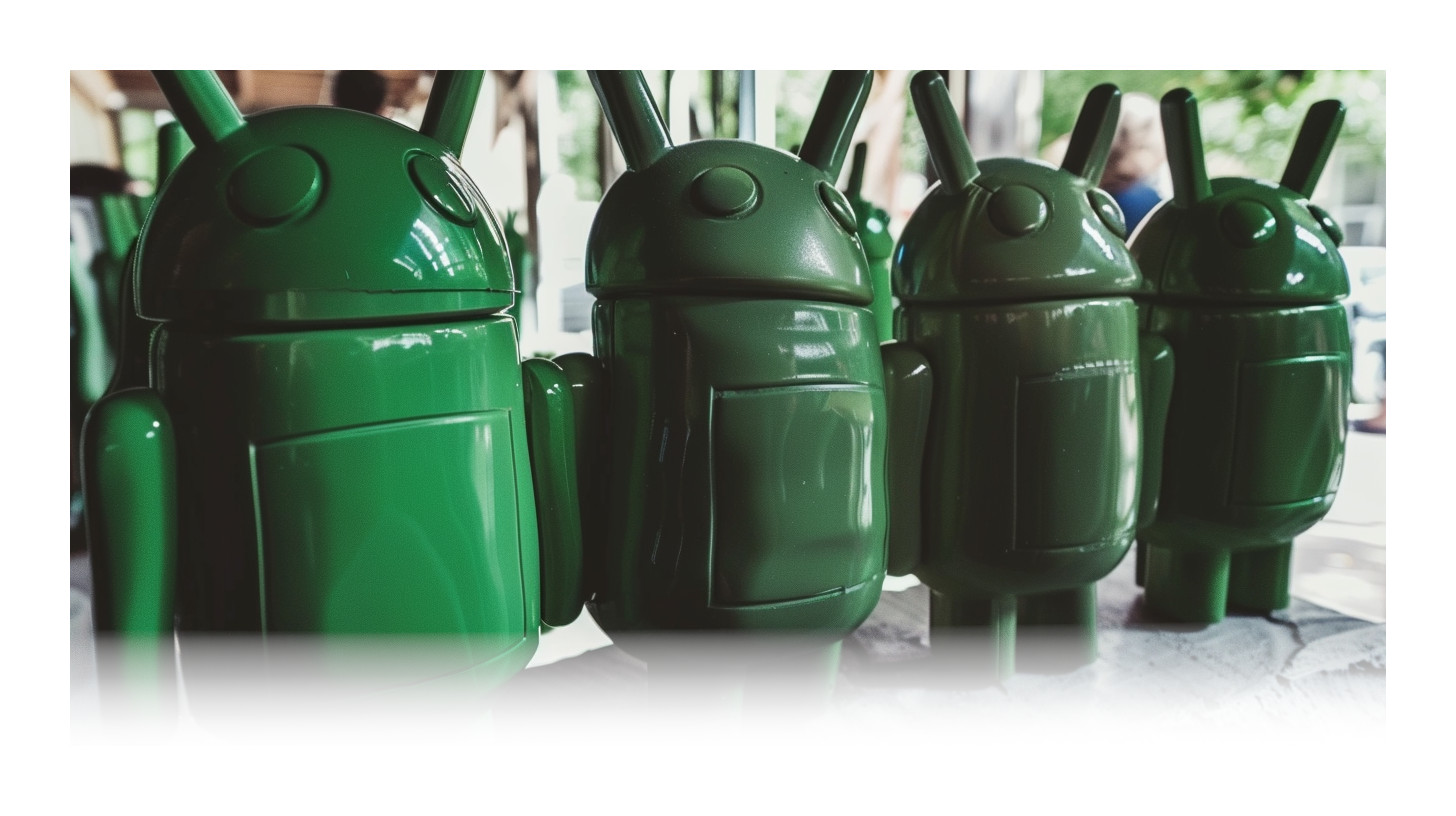
\includegraphics[width=\paperwidth]{./chapters/chapter-header-change-log.jpg}%
      }%
    }
  }

  \minitoc % Creating an actual minitoc mini lista contenuti

%  \section{Change Log}
%
%  \subsection{Firmware Change Log}

  \section{DWPS-13\_K04\_XMA311D2AV2-1\_A311D2\_8192M\_128G\_USBUART\_Airgo-0.0.0-20240611225217}
    \label{sec:firmware20240611225217}

  I had to disable com.xbh.share (AirgoCast v. \emph{\color{Grey}2.9.1.381.B}) to get the Wifi working. The firmware was periodically disconnecting every 2 minutes and 9 seconds\footnote{The disconnection frequency was calculated using the Python code in Listing\ref{lst:python-dhcp} and the accurate result is (2, 9.997571428571433)}. Figure \ref{fig:change-log} shows how frequent the disconnections were. The DhcpClient kept dropping down \textbf{onQuitting}.

  I went back to an even older firmware where the problem wasn't there but the screencasting app was super old.
  I removed the super old screencasting app. Installed com.xbh.share and the problem came back. I had to disable it again to get the Wifi working.
\clearpage
\lstinputlisting[language=Python, caption=Python code to calculate the disconnection frequency, label=lst:python-dhcp]{./chapters/change-log/dhcp-calc.py}

  \begin{figure}
    \centering
    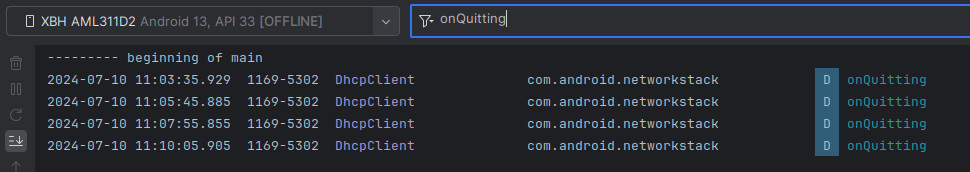
\includegraphics[width=0.9\textwidth]{./chapters/change-log/change-log.jpg}
    \caption{DHCP Client kept dropping down \textbf{onQuitting}}
    \label{fig:change-log}
  \end{figure}

  \section{DWPS-13\_K04\_XMA311D2AV2-1\_A311D2\_8192M\_128G\_USBUART\_Airgo-0.0.0-20240705151015}
    \label{sec:firmware20240705151015}

  The frequent disconnections is now fixed (AirgoCast v. \emph{\color{Grey}2.10.1.404.B}), but we noticed we couldn't see 2.4 Ghz signals easily.
  We had to manually determine the optimal Wi-Fi channel settings for the Akhter2\_4 network to ensure visibility and connectivity on the IFP.

  \begin{itemize}
    \item The router was set to the \textbf{Auto channel} mode.
    \item The Android IFP was able to detect and connect to the Akhter2\_4 network.
  \end{itemize}

  \paragraph{Testing on Channel 13}
  \begin{itemize}
    \item The router was manually set to \textbf{channel 13}.
    \item The Akhter2\_4 network became invisible on the Android device.
  \end{itemize}

  \paragraph{Reverting to Auto Channel}
  \begin{itemize}
    \item The router was reverted to \textbf{Auto channel} mode.
    \item Using the Net Analyzer app, it was determined that the router was operating on \textbf{channel 1}.
    \item With this setting, the Akhter2\_4 network was visible and accessible again on the Android device.
  \end{itemize}


  \paragraph{Channel 13 Visibility Issue}
  \begin{itemize}
    \item On 9th July 2024, having the router to channel 13\footnote{it's always been like this since my 1st day} allowed the Akhter2\_4 network to be visible and accessible on the Android device.
    \item On 10th July 2024, however, channel 13 prevents the Akhter2\_4 network from being seen by the Android device.
    \item This indicates a change in the network environment or interference on channel 13 that is now obstructing the visibility of Akhter2\_4.
  \end{itemize}

  \paragraph{Signal Strength Adjustment}
  \begin{itemize}
    \item Increasing the signal strength from medium to strong did not result in any improvement in the visibility of the Akhter2\_4 network on channel 13.
  \end{itemize}

  The tests indicate that while channel 13 was previously a viable option, it now poses an issue for network visibility on the Android device. The \textbf{Auto channel} setting, which defaults to \textbf{channel 1} in this environment, ensures that the Akhter2\_4 network remains visible and accessible. Signal strength adjustments did not mitigate the visibility issue on channel 13. Therefore, it is recommended to continue using the Auto channel setting to maintain reliable connectivity for the Akhter2\_4 network.

  \paragraph{Additional Tests}
  \begin{itemize}
    \item Channel 12: The WiFi is still not visible.
    \item Channel 11: The WiFi is visible.
  \end{itemize}

  There's a bug where the touch screen freezes on both firmwares (page \pageref{sec:firmware20240611225217} and page \pageref{sec:firmware20240705151015}).

  \paragraph{Channel Visibility Tests}
  \begin{itemize}
    \item Channel 10: Akhter2\_4 is visible on the unlocked screen close to production door with strong signal.
    \item Channel 9: Akhter2\_4 is visible on the unlocked screen close to production door but with weak signal. Visible on the locked-down screen in my corner.
    \item Channel 8: Akhter2\_4 is visible on the unlocked screen close to production door but with weak signal. Visible on the locked-down screen in my corner.
    \item Channel 7: Akhter2\_4 is visible on the unlocked screen close to production door but with weak signal. Visible on the locked-down screen in my corner.
    \item Channel 6: Akhter2\_4 is visible on the unlocked screen close to production door but with weak signal. Visible on the locked-down screen in my corner.
    \item Channel 5: Akhter2\_4 is visible on the unlocked screen close to production door but with weak signal. Visible on the locked-down screen in my corner.
    \item Channel 4: Akhter2\_4 is visible on the unlocked screen close to production door but with weak signal. Visible on the locked-down screen in my corner.
    \item Channel 3: Akhter2\_4 is visible on the unlocked screen close to production door but with weak signal. Visible on the locked-down screen in my corner.
    \item Channel 2: Akhter2\_4 is not visible on the unlocked screen close to production door. Visible on the locked-down screen in my corner but with one bar less.
    \item Channel 1: Akhter2\_4 has very weak signal on the unlocked screen close to production door and sometimes disappears. Very strong on the locked-down screen in my corner.
    \item Channel 13: Akhter2\_4 is not visible on the unlocked screen close to production door. Not visible on the locked-down screen in my corner.
  \end{itemize}

  At 11:53 on 10th July 2024 the Android IFP touch running the firmware shown on page \pageref{sec:firmware20240611225217} froze.
  At 12:36, we returned to Auto which is on channel 1. Akhter2\_4 is strongly visible on the unlocked screen close to production door and very weak and disappearing on the locked-down screen in my corner.

  At 12:09, I interacted with the screen with Touch frozen.
  At 12:22, I retouched the screen unlocked with log running.

  On 12th July at 11:39 the firmware shown on page \pageref{sec:firmware20240705151015} had the same old Wifi issue commented out in the video I've sent to Slin.
  The WiFi just stops connecting even to open Wifi. The only way to fix it is to restart the device.

  We have also noticed the Log doesn't create the folder when the log starts

  None of these problems are occurring with 5 GHz networks. All 16 channels have been tested and the results are consistent.



\part{APPENDICES}
\appendix
%\include{chapters/MyDevicePolicyManager}

%\glsaddall
\printglossary
\printindex
\end{document}
